

%  RAPPORT — PROJET SÉRIES CHRONOLOGIQUES
%  Université Nazi Boni — LSI — Année 2025-2026
%  Chargé de cours : Serge M.A. SOMDA, PhD.
% ============================================================


% ============================================================
%  SECTION 1 : CLASSE DU DOCUMENT ET OPTIONS GLOBALES
% ============================================================

\documentclass[
12pt,          % Taille de police
a4paper,       % Format du papier
oneside,       % Supprime les pages vierges entre chapitres
openright      % Les chapitres commencent toujours à droite
]{report}


% ============================================================
%  SECTION 2 : ENCODAGE ET LANGUE
% ============================================================

\usepackage[authoryear, round]{natbib}

\usepackage[utf8]{inputenc}
\usepackage[T1]{fontenc}
\usepackage[french]{babel}
\usepackage{csquotes}             % Requis avec babel/french


% ============================================================
%  SECTION 3 : POLICES ET TYPOGRAPHIE
% ============================================================

\usepackage{palatino}             % Police Palatino (élégante, académique)
\usepackage{microtype}            % Optimise l'espacement des caractères


% ============================================================
%  SECTION 4 : MISE EN PAGE
% ============================================================

\usepackage[
top=2.5cm,
bottom=2.5cm,
left=3cm,
right=2.5cm,
headheight=15pt
]{geometry}

\usepackage{setspace}
\onehalfspacing

\setlength{\parskip}{6pt}
\setlength{\parindent}{1.5em}


% ============================================================
%  SECTION 5 : COULEURS
% ============================================================

\usepackage[dvipsnames, table]{xcolor}

\definecolor{couleurPrimaire}{RGB}{0, 71, 130}
\definecolor{couleurblack}{RGB}{0, 0, 0}
\definecolor{couleurFond}{RGB}{245, 248, 252}
\definecolor{couleurSecondaire}{RGB}{198,40,40}
\definecolor{couleurTertiaire}{RGB}{27,120,80}
\definecolor{couleurGris}{RGB}{100,100,100}
\definecolor{couleurOr}{RGB}{180,130,20}


% ============================================================
%  SECTION 6 : EN-TÊTES ET PIEDS DE PAGE
% ============================================================

% ============================================================
%  SECTION 6 : EN-TÊTES ET PIEDS DE PAGE
% ============================================================

\usepackage{fancyhdr}
\pagestyle{fancy}
\fancyhf{}

% Document oneside → positions L et R uniquement
\fancyhead[L]{%
	\small\textcolor{couleurGris}{%
		Fonction Enseignement %
	}%
}
\fancyhead[R]{%
	\small\textcolor{couleurGris}{\nouppercase{\leftmark}}%
}
\fancyfoot[C]{%
	\textcolor{couleurGris}{\thepage}%
}

% Supprimer la ligne d'en-tête sur les pages de chapitre
\fancypagestyle{plain}{%
	\fancyhf{}%
	\fancyfoot[C]{\textcolor{couleurGris}{\thepage}}%
	\renewcommand{\headrulewidth}{0pt}%
}


% ============================================================
%  SECTION 7 : STYLE DES CHAPITRES ET TITRES
% ============================================================

\usepackage{titlesec}
\usepackage{titletoc}

% --- Style des CHAPITRES ---
\titleformat{\chapter}[display]
{\normalfont\bfseries\color{white}}
{%
	\colorbox{couleurPrimaire}{%
		\parbox{\dimexpr\textwidth+2\fboxsep\relax}{%
			\vspace{6pt}
			\hspace{10pt}
			\Large\color{white}
			\chaptertitlename~\thechapter
			\vspace{6pt}
		}%
	}%
}
{0pt}
{%
	\colorbox{couleurSecondaire!20}{%
		\parbox{\dimexpr\textwidth+2\fboxsep\relax}{%
			\vspace{8pt}
			\hspace{10pt}
			\huge
			\vspace{8pt}
		}%
	}%
	\vspace{-\baselineskip}
	\huge\color{couleurPrimaire}
}
[\vspace{10pt}\color{couleurPrimaire}\hrule\vspace{20pt}]

% --- Style des SECTIONS ---
\titleformat{\section}
{\normalfont\Large\bfseries\color{couleurPrimaire}}
{\thesection}{1em}{}
[\vspace{2pt}{\color{couleurPrimaire!40}\titlerule[0.5pt]}]

% --- Style des SOUS-SECTIONS ---
\titleformat{\subsection}
{\normalfont\large\bfseries\color{couleurblack}}
{\thesubsection}{1em}{}

% --- Style des SOUS-SOUS-SECTIONS ---
\titleformat{\subsubsection}
{\normalfont\normalsize\bfseries\color{couleurblack}}
{\thesubsubsection}{1em}{}

% --- Espacement autour des titres ---
\titlespacing*{\chapter}{0pt}{0pt}{30pt}
\titlespacing*{\section}{0pt}{20pt}{8pt}
\titlespacing*{\subsection}{0pt}{15pt}{6pt}
\titlespacing*{\subsubsection}{0pt}{10pt}{4pt}


% ============================================================
%  SECTION 8 : TABLEAUX ET FIGURES
% ============================================================
\usepackage{tcolorbox}
\tcbuselibrary{skins}
\usepackage{array}
\usepackage{booktabs}
\usepackage{tabularx}
\usepackage{graphicx}
\usepackage{float}
\usepackage{multirow}
\usepackage{multicol}
\usepackage{caption}
\usepackage{subcaption}
\usepackage{longtable}

\captionsetup{
	font=small,
	labelfont={bf, color=couleurPrimaire},
	labelsep=period,
	justification=centering
}

\graphicspath{{../Output/figures/}}


% ============================================================
%  SECTION 9 : MATHÉMATIQUES
% ============================================================

\usepackage{amsmath, amssymb, amsthm}


% ============================================================
%  SECTION 10 : LIENS HYPERTEXTES
% ============================================================

\usepackage[
colorlinks = true,
linkcolor  = couleurPrimaire,
citecolor  = couleurTertiaire,
urlcolor   = couleurPrimaire
]{hyperref}


% ============================================================
%  SECTION 11 : LISTES
% ============================================================

\usepackage{enumitem}
\usepackage{url}


% ============================================================
%  SECTION 12 : TABLE DES MATIÈRES PERSONNALISÉE
% ============================================================

\usepackage{tocloft}
\renewcommand{\cftchapfont}{\bfseries\color{couleurPrimaire}}
\renewcommand{\cftsecfont}{\color{couleurblack}}


% ============================================================
%  COMMANDES PERSONNALISÉES
% ============================================================

\newcommand{\IHPC}{\textit{IHPC}}
\newcommand{\EQM}{\textit{EQM}}


% ============================================================
%  DÉBUT DU DOCUMENT
% ============================================================

\begin{document}
	
	
% ============================================================
%  PAGE DE GARDE (PAGE 1)
% ============================================================


% ============================================================
%  PAGE DE TITRE
% ============================================================
% ============================================================
%  PAGE DE GARDE
% ============================================================

% ============================================================
%  PAGE DE GARDE
% ============================================================

\begin{titlepage}
	\thispagestyle{empty}
	
	% ── Bandeau supérieur bleu ────────────────────────────────
	\noindent
	\colorbox{couleurPrimaire}{%
		\parbox{\dimexpr\textwidth\relax}{%
			\vspace{10pt}
			\centering
			{\small\bfseries\color{white}
				BURKINA FASO\\[2pt]
				Unité --- Progrès --- Justice
			}
			\vspace{10pt}
		}%
	}
	
	\vspace{0.5cm}
	
	% ── Logos et intitulés ────────────────────────────────────
	\noindent
	\begin{minipage}[t]{0.48\textwidth}
		\centering
		
\includegraphics[width=2.2cm]{logo_bf.png}\\[6pt]
		{\footnotesize\scshape
			Ministère de l'Enseignement\\
			Supérieur, de la Recherche\\
			et de l'Innovation
		}
	\end{minipage}
	\hfill
	\begin{minipage}[t]{0.48\textwidth}
		\centering
		
\includegraphics[width=2.2cm]{logo_unb.png}\\[6pt]
		{\footnotesize\scshape
			Université Nazi Boni\\[3pt]
			UFR Sciences Exactes\\
			et Appliquées\\[3pt]
			Licence Statistiques\\
			et Informatique \\
				
		}
	\end{minipage}
	
	\vspace{0.6cm}
	
	% ── Filet séparateur ──────────────────────────────────────
	{\color{couleurPrimaire}\rule{\linewidth}{1pt}}
	
	
	\vspace{0.5cm}
	
	% ── Type de document ─────────────────────────────────────
	\begin{center}
		{\large\bfseries\color{couleurGris}
			
			RAPPORT DE PROJET
		}\\[4pt]
		{\small\itshape Sur le thème :}
	\end{center}
	
	\vspace{0.4cm}
	
	% ── Titre encadré ─────────────────────────────────────────
	\begin{tcolorbox}[
		enhanced,
		colback  = couleurPrimaire!8,
		colframe = couleurPrimaire,
		boxrule  = 1pt,
		arc      = 6pt,
		left     = 10pt,
		right    = 10pt,
		top      = 8pt,
		bottom   = 8pt
		]
		\begin{center}
			{\large\bfseries\color{couleurPrimaire}
				Analyse de l'Indice Harmonisé des Prix\\
				à la Consommation :\\[4pt]
				Secteur des Services d'Enseignement\\
				au Burkina Faso (2015--2025)
			}
		\end{center}
	\end{tcolorbox}
	
	\vspace{0.6cm}
	
	% ── Auteurs ───────────────────────────────────────────────
	\begin{center}
		{\small\itshape Présenté par les membres du groupe 11 :}\\[8pt]
		{\large\bfseries\color{couleurPrimaire}
			SAKO Biton F.B. Cherif\\[4pt]
			OUATTARA Basoungalo J. Ulrich
		}\\[4pt]
		{\small\color{couleurGris}
			Étudiants en Licence 2 --- Statistiques et Informatique
		}
	\end{center}
	
	\vspace{0.5cm}
	
	% ── Filet séparateur ──────────────────────────────────────
	{\color{couleurPrimaire}\rule{\linewidth}{0.5pt}}
	
	\vspace{0.4cm}
	
	% ── Encadrant et période ──────────────────────────────────
	\noindent
	\begin{minipage}[t]{0.48\textwidth}
		{\small
			\textbf{\underline{Chargé du cours :}}\\[5pt]
			Serge M.A. SOMDA, PhD\\
			{\color{couleurGris}\itshape
				\textbf{Année académique 2025--2026}
			}
		}
	\end{minipage}
	\hfill
	\begin{minipage}[t]{0.48\textwidth}
		\raggedleft
		{\small
			\textbf{\underline{Période du projet :}}\\[5pt]
			22 Mars 2026 --- 10 Avril 2026
		}
	\end{minipage}
	
	\vfill
	

				
			
	
\end{titlepage}
	
	% ============================================================
	%  TABLE DES MATIÈRES
	% ============================================================
	
	\tableofcontents
	\newpage
	
	
		% --- LISTE DES ABRÉVIATIONS ---
	\chapter*{Liste des abr\'eviations}
	\addcontentsline{toc}{chapter}{LISTE DES ABR\'EVIATIONS}
	\markboth{LISTE DES ABR\'EVIATIONS}{LISTE DES ABR\'EVIATIONS}
	
	\begin{tabbing}
		\hspace{4cm} \= \kill   % Définit la largeur de la colonne gauche
		% <-- FORMAT : SIGLE \> Signification complète \\
		\textbf{LSI}  \> Licence Statistique-Informatique \\[3pt]
		 \textbf{ACF}      \> Fonction d'Autocorrélation \\[3pt]
		\textbf{ADF}      \> Augmented Dickey-Fuller \\[3pt]
		\textbf{AIC}      \> Critère d'Information d'Akaike \\[3pt]
		\textbf{ARIMA}    \> AutoRegressive Integrated Moving Average \\[3pt]
		\textbf{BIC}      \> Critère d'Information Bayésien \\[3pt]
		\textbf{BCEAO}    \> Banque Centrale des États de l'Afrique de l'Ouest \\[3pt]
		\textbf{CITE-97}  \> Classification Internationale Type de l'Éducation (1997) \\[3pt]
		\textbf{COICOP}   \> Classification de la Consommation Individuelle par Objectif \\[3pt]
		\textbf{COVID-19} \> Coronavirus Disease 2019 \\[3pt]
		\textbf{EQM}      \> Erreur Quadratique Moyenne \\[3pt]
		\textbf{IHPC}     \> Indice Harmonisé des Prix à la Consommation \\[3pt]
		\textbf{IIEP}     \> Institut International de Planification de l'Éducation \\[3pt]
		\textbf{INSD}     \> Institut National de la Statistique et de la Démographie \\[3pt]
		\textbf{ISBLSM}   \> Institutions Sans But Lucratif au Service des Ménages \\[3pt]
		\textbf{MENAPLN}  \> Ministère de l'Éducation Nationale, de l'Alphabétisation \\[3pt]
		\> et de la Promotion des Langues Nationales \\[3pt]
		\textbf{NCOA}     \> Nomenclature de Consommation Ouest-Africaine \\[3pt]
		\textbf{NCOA-IHPC}\> Nomenclature de Consommation Ouest-Africaine \\[3pt]
		\> adaptée pour l'IHPC \\[3pt]
		\textbf{PACF}     \> Fonction d'Autocorrélation Partielle \\[3pt]
		\textbf{PER}      \> Projet d'Éducation par la Radio \\[3pt]
		\textbf{SARIMA}   \> Seasonal AutoRegressive Integrated Moving Average \\[3pt]
		\textbf{SCN}      \> Système de Comptabilité Nationale \\[3pt]
		\textbf{UEMOA}    \> Union Économique et Monétaire Ouest-Africaine \\[3pt]
		\textbf{UNESCO}   \> Organisation des Nations Unies pour l'Éducation, \\[3pt]
		\> la Science et la Culture \\[3pt]
		\textbf{UNICEF}   \> Fonds des Nations Unies pour l'Enfance \\[3pt]
		\textbf{PDDEB}   \> Plan Décennal de Développement de l’Éducation de Base \\[3pt]
		\textbf{PSE}   \> Programme Sectoriel de l’Éducation \\[3pt]
		\textbf{IDR}   \> Institut de Recherche pour le Développement \\[3pt]
		
		% <-- AJOUTER VOS ABRÉVIATIONS
	\end{tabbing}
	
	\newpage
	
	
	
	\listoffigures
	\addcontentsline{toc}{chapter}{Liste des figures}
	\newpage
	
	\listoftables
	\addcontentsline{toc}{chapter}{Liste des tableaux}
	\newpage
	
	
	
	% ============================================================
	%  INTRODUCTION
	% ============================================================
	
	\chapter*{Introduction}
	\addcontentsline{toc}{chapter}{Introduction}
	\markboth{Introduction}{Introduction}
	
	Le Burkina Faso, à l’instar de nombreux pays d’Afrique subsaharienne, a inscrit la réduction des frais liés aux services éducatifs et l’accès universel à l’éducation dans ses stratégies nationales de développement. Cette orientation vise à permettre aux ménages, y compris les plus défavorisés, de faire face aux coûts de scolarisation et de garantir une éducation pour tous. Depuis l’indépendance en 1960, cette ambition s’est traduite par de nombreuses études, plans sectoriels et réformes successives. Toutefois, malgré ces efforts, les objectifs d’un système éducatif inclusif et financièrement accessible peinent à être pleinement atteints, et les ménages continuent de supporter une charge importante.
	Plusieurs mesures ont été mises en œuvre pour alléger cette pression financière : octroi de bourses d’études, incitations aux établissements privés à revoir leurs tarifs à la baisse, et réformes structurelles telles que celle du continuum éducatif en 2017. Malgré ces initiatives, les coûts des services éducatifs restent élevés, et les ménages continuent d’en payer le prix, parfois au détriment d’autres besoins essentiels. Cette tendance s’est accentuée au cours de la dernière décennie (2015–2025), dans un contexte marqué par des crises sanitaires, sécuritaires et économiques.
	Afin de mieux comprendre cette dynamique inflationniste, nous nous intéresserons à l’évolution de l’Indice Harmonisé des Prix à la Consommation (IHPC) appliqué aux services d’enseignement. Cette composante de l’IHPC permet d’analyser les variations des prix dans le secteur éducatif et d’évaluer leur impact sur les ménages burkinabè.
	L’objectif principal de cette étude est d’analyser et de modéliser l’évolution mensuelle de l’indice considéré, afin de produire des prévisions à court terme. Pour atteindre cet objectif, trois approches méthodologiques complémentaires ont été mobilisées : le lissage exponentiel, la décomposition classique des séries temporelles et la modélisation ARIMA. Cette combinaison permet de confronter des méthodes de nature différente et d’évaluer leur pertinence respective dans le contexte étudié.
	
	
	
	
	% Présenter ici :
	% - Le contexte : l'IHPC au Burkina Faso, rôle de l'INSD
	% - L'intérêt d'étudier le secteur de l'enseignement
	% - Les objectifs du rapport
	% - Le plan du rapport
	
	\newpage
	
	
	% ============================================================
	%  CHAPITRE 1 — DESCRIPTION DE LA SÉRIE
	% ============================================================
	
	\chapter{Description de la série chronologique}
	
	\section{L'indice harmonisé des prix à la consommation (Définition et Construction)}
	\subsection{Définition de l'\IHPC{}}
	

	% Qu'est-ce que l'IHPC ? Base 100 en 2023.
	% Méthodologie UEMOA. Rôle de l'INSD.
		L'IHPC (Indice Harmonisé des Prix à la Consommation) est un indicateur économique
	qui mesure l'évolution des prix des biens et services consommés par les ménages. Il
	est utilisé pour suivre l'inflation et orienter les décisions économiques. L'IHPC est
	basé sur une enquête auprès des ménages et des prix des produits auprès des
	commerçants, avec une couverture géographique qui inclut toutes les régions du Burkina FASO \citep{insd2025}. 
	
	Autrement dit: L'\IHPC{} est un indicateur de suivi de l'évolution des prix permettant de déterminer si cette évolution est inflationniste ou déflationniste...
	Il est construit avec une base de référence égale à 100 : une valeur 
	supérieure à 100 indique une tendance à la hausse des prix, tandis qu'une 
	valeur inférieure signale une tendance à la baisse \citep{lefaso2025}.
	
	Cet indice, harmonisé car le même instrument de suivi de l'évolution des prix a été mis en place dans les pays membres de l'Union Economique et Monétaire Ouest-Africaine (UEMOA). Il a satisfait à un critère important de 
	qualité du point de vue de la couverture géographique. En effet, l'\IHPC{} a pour couverture géographique les treize (13) régions administratives du pays et pour population de référence l'ensemble des ménages de ces 13 régions. Le 
	panier de la ménagère comprend environ 838 produits suivis dans 3951 points d'observation. Plus de 25000 relevés de prix sont effectués chaque mois par les enquêteurs de l'INSD. La période de base de l'IHPC est l'année 2023 et 
	les pondérations de l'indice proviennent d'une enquête sur les dépenses des ménages réalisée en 2021 .Cette nomenclature comporte \textbf{14 fonctions} \citep{insd2025}.
	
	Les dépenses couvertes sont classées selon la Nomenclature de 
	Consommation Ouest-Africaine adaptée pour l'\IHPC{} (NCOA-IHPC), 
	dérivée de la Classification de la Consommation Individuelle par 
	Objectif (COICOP). Cette dernière est une classification fonctionnelle 
	utilisée dans le Système de Comptabilité Nationale (SCN 1993) et porte 
	sur les dépenses de consommation individuelle de trois secteurs 
	institutionnels : les ménages, les institutions sans but lucratif au 
	service des ménages (ISBLSM) et les administrations publiques 
	\citep{afristat2022ncoa}.
	Une adaptation de cette nomenclature internationale à la zone UEMOA 
	a été réalisée sous l'appellation Nomenclature de Consommation 
	Ouest-Africaine (NCOA), en y introduisant un quatrième niveau appelé 
	\textit{postes de consommation}. La NCOA-IHPC, dérivée de la NCOA, 
	définit l'ensemble des indices harmonisés des prix à la consommation 
	devant être calculés par les instituts nationaux de statistique des 
	États membres de l'UEMOA. Elle comprend \citep{afristat2022ncoa} :
	\begin{itemize}
		\item 12 fonctions de consommation ;
		\item 41 groupes ;
		\item 78 sous-groupes ;
		\item 126 postes de consommation.
	\end{itemize}
	
		
	
\subsection{Construction de l'\IHPC{}}

L'\IHPC{} repose sur le principe de l'\textbf{indice de Laspeyres}, 
qui mesure la variation des prix entre une période de base $0$ et une 
période courante $t$, en maintenant les quantités consommées constantes 
à leur niveau de la période de base. Formellement, si l'on considère 
$M$ biens et services, l'indice de Laspeyres s'écrit \citep{afristat2022} :

\begin{equation}
	I_{t/0} = 100 \times \frac{\displaystyle\sum_{i} P_{it}\, Q_{i0}}
	{\displaystyle\sum_{i} P_{i0}\, Q_{i0}}
	\label{eq:laspeyres}
\end{equation}

où $P_{i0}$ et $P_{it}$ désignent respectivement le prix du bien $i$ 
à la période de base et à la période courante, et $Q_{i0}$ la quantité 
échangée du bien $i$ à la période de base.

Cette formule peut être réécrite sous une forme équivalente faisant 
apparaître les \textit{coefficients budgétaires} ou \textit{pondérations} 
$\Omega_{i0}$ et les indices élémentaires $I_{i/0}$ \citep{afristat2022} :

\begin{equation}
	I_{t/0} = 100 \times \sum_{i} \Omega_{i0} \times \frac{P_{it}}{P_{i0}}
	= 100 \times \sum_{i} \Omega_{i0} \times I_{i/0}
	\label{eq:laspeyres2}
\end{equation}

avec :
\begin{equation}
	\Omega_{i0} = \frac{P_{i0}\, Q_{i0}}{\displaystyle\sum_{i} P_{i0}\, Q_{i0}}
	\label{eq:ponderations}
\end{equation}

Chaque pondération $\Omega_{i0}$ représente la part de la dépense 
consacrée au bien $i$ dans la consommation totale des ménages à la 
période de base. Ces coefficients sont estimés à l'aide d'une 
\textbf{enquête budget-consommation} réalisée à la période de base, 
complétée par d'autres sources statistiques exogènes \citep{afristat2022}.

La mise en \oe{}uvre concrète de cet indice repose sur trois éléments 
fondamentaux \citep{afristat2022} :

\begin{itemize}
	\item \textbf{Un échantillon de biens et services} représentatif 
	de la consommation des ménages, structuré selon la nomenclature 
	NCOA-IHPC en fonctions, groupes, sous-groupes, postes et variétés ;
	
	\item \textbf{Un échantillon de points de vente} dans lesquels 
	les prix sont relevés, constitué dans chaque strate de points de 
	vente définie sur la zone d'enquête ;
	
	\item \textbf{Un échantillon de dates de relevés} permettant 
	d'estimer les prix pratiqués au cours du mois en cours.
\end{itemize}

Au Burkina Faso, les prix de base des biens et services sont déterminés 
par observation directe sur une période de base relativement longue (10ans). 
Les prix du mois en cours proviennent soit d'observations réalisées 
durant le mois, soit d'observations effectuées à d'autres périodes 
\citep{afristat2022}. La période de base retenue pour l'\IHPC{} 
du Burkina Faso est l'année \textbf{2023}, les pondérations étant 
issues d'une enquête sur les dépenses des ménages réalisée en 
\textbf{2021} \citep{insd2025}.
	
	
	\section{Description de la fonction Enseignement}
	% Définition du chapitre "Enseignement" dans la nomenclature UEMOA.
	% Composantes : frais de scolarité, fournitures, etc.
	% Intérêt économique et social.
\subsection{L'\IHPC{} du secteur de l'Enseignement}

Dans la NCOA-IHPC, la \textbf{fonction 10} est consacrée aux services 
d'enseignement. Elle constitue l'une des 12 fonctions de consommation 
de la nomenclature et porte le code \textbf{10 --- ENSEIGNEMENTS}. Subdivisée en quatre groupes (\citep{afristat2022ncoa}), cette fonction ne contient \textbf{que des services}, et non des produits physiques. Ce qui lui donne de la valeur, sont principalement les \textbf{frais de scolarité} composés de  \textbf{frais d'inscription, les frais de scolarité proprement dits et les droits d'examen} à chaque niveau d'enseignement y compris la téléenseignement. En annexe, les répétitions privées payantes même avec un poids faible donne également de la valeur à la dite fonction.

\begin{itemize}
	\item \textbf{10.1} --- Enseignement préélémentaire et primaire : frais 
	d'inscription et de scolarité à la maternelle et au primaire, 
	programmes d'alphabétisation pour les élèves trop âgés pour 
	s'inscrire à l'école primaire (niveaux 0 et 1 de la CITE-97)  ;
	
	\item \textbf{10.2} --- Enseignement secondaire: frais de scolarité au 
	collège (post-primaire) et au lycée, y compris l'enseignement 
	secondaire extrascolaire dispensé aux adultes et aux jeunes 
	(niveaux 2 et 3 de la CITE-97) ;
	
	\item \textbf{10.4} --- Enseignement supérieur : frais d'inscription à 
	l'université, dans les grandes écoles et instituts supérieurs 
	(niveaux 5 et 6 de la CITE-97)  ;
	
	\item \textbf{10.5} --- Enseignement postsecondaire non supérieur 
	et enseignement non défini par niveau : formations professionnelles payantes et cours de culture 
	générale destinés aux adultes (niveau 4 de la CITE-97).
	
	\citep{afristat2022ncoa}
\end{itemize}

Il convient de préciser que cette fonction couvre \textit{exclusivement} 
les services d'enseignement, organisés selon les catégories définies 
dans la Classification Internationale Type de l'Éducation établie en 
1997 (CITE-97) par l'UNESCO. Elle exclut ainsi les matériels 
pédagogiques tels que les livres (09.5.1) et la papeterie (09.5.4), 
les services de santé (06), de transport (07.3), de restauration 
(11.1.2) et d'hébergement (11.2.0). Elle comprend en revanche le 
téléenseignement, notamment dispensé par radio et télévision 
\citep{afristat2022ncoa}. Ce mode d'enseignement a pris une importance particulière au Burkina Faso dans le contexte de crise sécuritaire. En juillet 2021, l'UNICEF 
rapportait que le Projet d'Éducation par la Radio (PER) avait permis de mobiliser plus de 400 enfants dans des clubs d'écoute, certains d'entre eux ayant même pu obtenir leur Certificat d'Études Primaires (CEP) grâce à cette intervention \citep{unicef2021radio}.

Au sein du panier global de l'\IHPC{}, la division 
\textit{Services d'enseignement} porte une pondération de 
\textbf{238 pour 10 000}, soit \textbf{2,38\,\%} du panier total. 
Le tableau~\ref{tab:ponderations} présente la place de cette division 
par rapport aux autres fonctions de consommation.

\begin{table}[H]
	\centering
	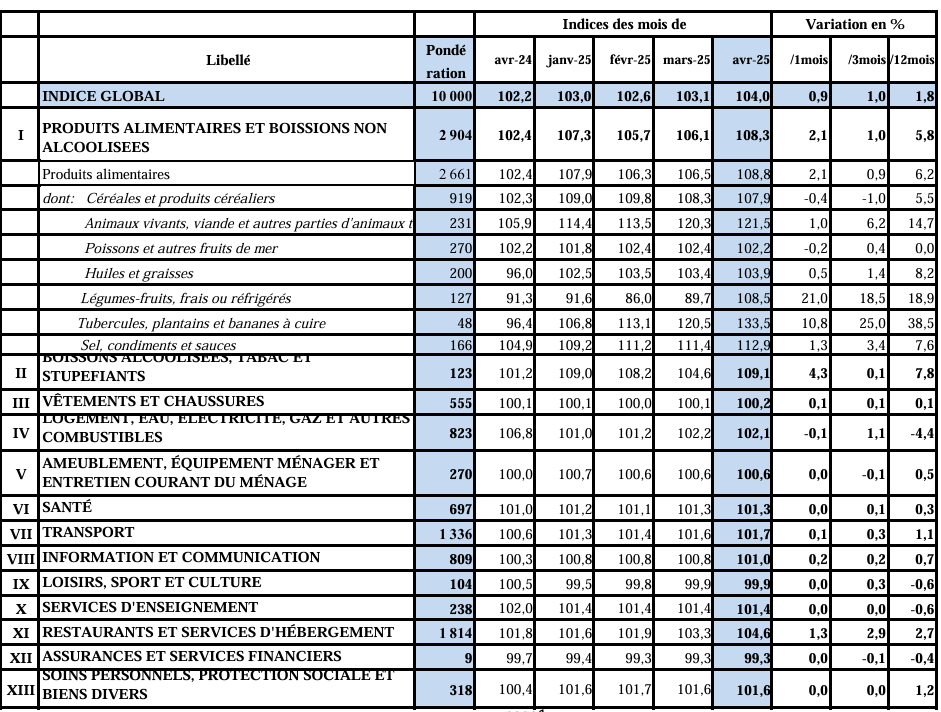
\includegraphics[width=0.95\textwidth]{tab_ponderations}
	\caption{Pondérations des divisions de l'\IHPC{} au Burkina Faso
		(Base 100 en 2023)}
	\label{tab:ponderations}
	\small\textit{Source : INSD \citep{insd2025}}
\end{table}

La pondération de la division des \textit{Services d'enseignement} qui est de \textbf{2,38\,\%}, aussi modeste soit elle, est d'une importance sociale et politique au Burkina FASO. En effet, toute variation des prix des services d'enseignement affecte directement le budget des ménages, en particulier les plus vulnérables pour qui l'accès à l'éducation constitue déjà un défi majeur. 

\subsection{Description de la fonction}

L’évolution de l’IHPC des services d’enseignement au Burkina Faso illustre une tendance haussière de long terme, ponctuée de chocs liés aux réformes éducatives, aux crises économiques, aux changements politiques et aux événements sécuritaires. Durant la période coloniale et les premières années postindépendance, l’État assumait l’essentiel des dépenses, mais l’accès restait limité à une élite \citep {sore2014logiques}. Les réformes de ruralisation et communautaire des années 1970 ont cherché à adapter l’école aux réalités rurales, mais faute de moyens, une partie des charges a été transférée aux familles\citep {sore2014logiques}.
La période révolutionnaire (1983–87) a mobilisé des ressources publiques et communautaires pour l’alphabétisation, mais la crise économique et les ajustements structurels de la fin des années 1980 ont réduit drastiquement les budgets éducatifs, entraînant une déscolarisation et une hausse des frais privés \citep {sore2014logiques}.
Dans les années 1990, la reprise grâce aux bailleurs s’est accompagnée de conditions qui imposaient une rationalisation budgétaire, tandis que les ménages voyaient croître leurs dépenses\cite{Pilon2004}.
Le PDDEB (2000–2009) a marqué une hausse des investissements publics, avec construction d’écoles et recrutement d’enseignants contractuels, mais les coûts indirects pour les ménages sont restés élevés \cite{INSD2001}.
Le PSE (2010–2020) a favorisé la diversification et la montée du privé, accentuant la charge financière des familles.
 L’INSD montre que les dépenses éducatives absorbent une part croissante du budget des ménages, avec de fortes disparités entre zones urbaines et rurales \cite{INSD2001}.

À partir de 2015, l’IHPC suit une tendance haussière mais ponctuée de chocs. En 2017, une baisse drastique est observée : elle correspond à la réforme du curriculum qui a rationalisé les contenus et réduit certains coûts pédagogiques, notamment en fusionnant des matières et en simplifiant les charges pour les familles \cite{INSD2001}.
En 2018, une hausse est enregistrée avec la mise à jour des certifications et diplômes, qui a entraîné des frais supplémentaires pour les examens et une augmentation des coûts administratifs.
En 2021, un pic marqué apparaît, lié aux effets post COVID 19 : la pandémie a imposé des dépenses exceptionnelles pour le téléenseignement, les équipements numériques et les mesures sanitaires, ce qui a gonflé l’indice \cite{unicef2021radio}.
À cela s’ajoute la crise sécuritaire avec la montée des attaques terroristes dans le nord et l’est du pays, qui a fragilisé l’accès à l’école, entraînant des coûts supplémentaires pour sécuriser les établissements et déplacer des élèves, accentuant la pression sur les budgets publics et privés.
 En 2022–2023, les changements de régime politique et l’adoption de nouvelles feuilles de route éducatives ont entraîné des réorientations budgétaires, parfois au détriment de la stabilité des coûts.
Enfin, en 2024, une baisse post pédagogique est observée, conséquence des ajustements introduits après 2023 : rationalisation des TIC, introduction de cantines endogènes et meilleure intégration des innovations pédagogiques, ce qui a réduit certains coûts 

L’allure générale de la courbe IHPC est donc une ligne ascendante ponctuée de variations nettes : une chute en 2017, un rebond en 2018, un sommet en 2021, une correction en 2024. Cette dynamique illustre la tension constante entre ambitions nationales, prescriptions internationales et contraintes économiques, mais aussi l’impact des faits historiques : crises économiques, changements de régime avec nouvelles orientations éducatives, et insécurité liée aux attaques terroristes qui augmentent les coûts de fonctionnement et fragilisent l’accès. L’État finance les grandes réformes et infrastructures, tandis que les ménages assument une part croissante des frais quotidiens, accentuant les inégalités sociales et territoriales.





 \section{Visualisation de la série et argumentation de son évolution}
 
 \begin{figure}[H]
 	\centering
 	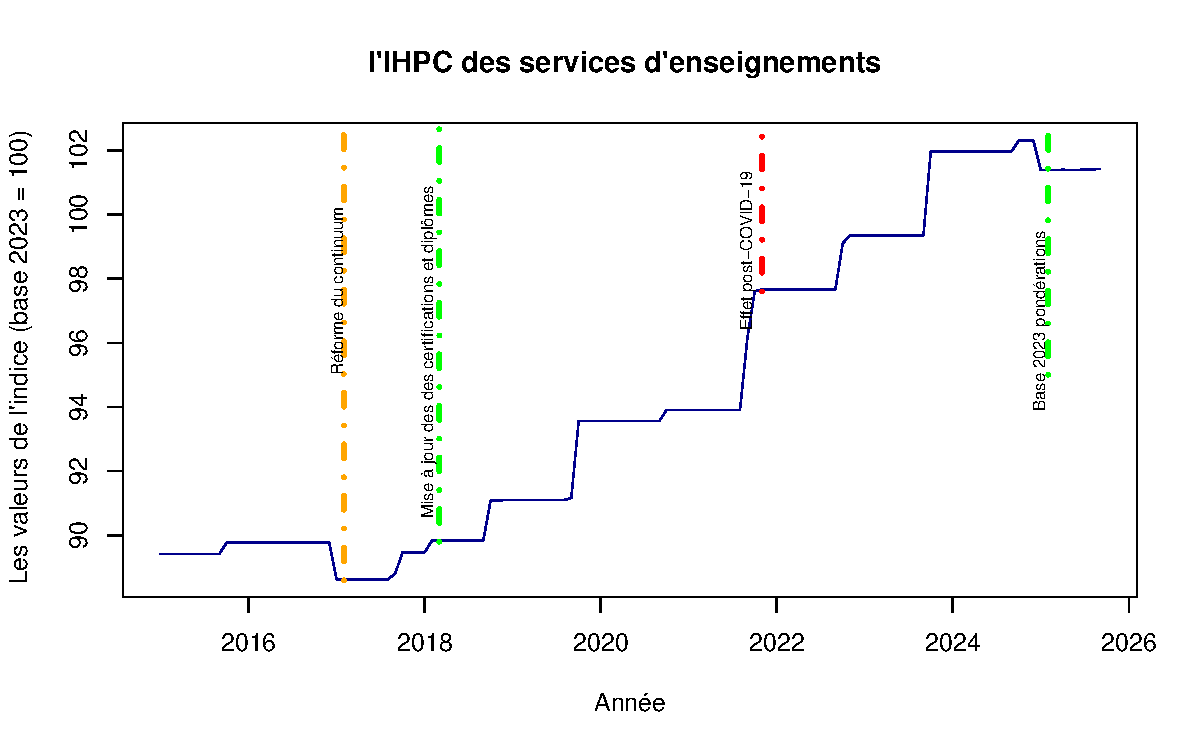
\includegraphics[width=0.95\textwidth]{graphe_serie_brute-1}
 	\caption{Visualisation de la série brute}
 	\label{fig:serie_brute}
 \end{figure}
 
 L'observation de la fonction  \textit{Services d'enseignement} met premièrement en évidence une baisse marquée de l'\IHPC{} entre \textit{décembre 2016} et \textit{janvier 2017}, période fortement influencée par la réforme du continuum d’éducation de base qui visait à mutualiser les ressources humaines et matérielles et à réduire les coûts pour les familles, notamment par des subventions et des mesures de gratuité dans certaines zones rurales \citep{unesco}. Les attaques terroristes de janvier 2016 à Ouagadougou, bien que constituant un choc sécuritaire majeur, n'ont pas eu d'effet mesurable sur les prix des services d'enseignement, l'indice étant resté stable à 89,77 tout au long de l'année. 
 
 De \textit{janvier -février 2018} nous constatons un petit saut de l'indice au cours de l'année scolaire, un saut dû à la mise à jour des certifications et diplômes, qui a entraîné des frais supplémentaires pour les examens et une augmentation des coûts administratifs.
 
 Après ces évènements, on commence à constaté une tendance haussière de l’IHPC  des \textit{Services d'enseignement} avec des cycles répétitifs nettement visible à l'œil nu. En effet, de \textit{2018 à 2025}, la situation sécuritaire du pays devient très instable dû à l'amplification des attaques terroristes. Cette situation entraina la fermeture des plusieurs écoles et un déplacement massif de la populations des zones concernées. D'après l'\textit{UNICEF}, dans un rapport publié en \textit{2024}, le \textit{sahel}, où la crise a débuté en 2019 comptait plus de \textbf{90\,\%} de ses écoles fermées. La région de l’Est et la Boucle du Mouhoun, voyait le nombre d’écoles fermées fortement augmenté à partir de 2021-22 et où plus de \textbf{60\,\%} des écoles sont maintenant fermées, et enfin les régions du Centre-Nord et du Nord, où \textbf{40 à 50\,\%}des écoles sont maintenant fermées \citep{unicef2025dms}. La combinaison de fermetures des classes, les déplacements, et les saturation causées par la demande forte des élèves déplacés ont entrainé une hausse des frais de scolarité ce qui a provoqué une pression haussière durable sur l’indice des services éducatifs sur cette période.
 
 Lors de son évolution, on remarque une montée exponentielle entre \textit{juillet-octobre 2021}. En effet, la reprise des classes après les perturbations liées à la pandémie de la \textit{COVID-19}, l'aggravation des attaques et les fermetures d’établissements ,à la rentrée scolaire 2021 a entraîné une hausse des frais de scolarité. Cette reprise a directement gonflé l’indice de la fonction \textit{Enseignement}.
 Le renversement du pouvoir de Mr Roch Kabore en \textit{janvier 2022} et celui du LCL Damiba en  \textit{septembre 2022} n'a pas eu de répercutions direct sur l'indice des \textit{Services d'enseignement}. En effet, l'indice est resté constant tout u long de l'année scolaire :  \textit{octobre- juillet 2022}.  Cependant, \textbf{en 2023}, en plus des déplacements interne accrus qui entrainèrent une saturation des écoles urbaines, l’adoption de nouvelles feuilles de route éducatives dû aux changement de régimes qui ont entraîné des réorientations budgétaires,  ont causé une augmentation des frais de scolarité tout au long de l'année ce qui entraina un saut positif significatif de l'\IHPC{} le faisant passé la barre des 100 à la rentré scolaire 2023-2024.
 Sur la période de \textit{novembre 2024} à \textit{janvier 2025}, on observe une baisse de l'indice. Une baisse qui tire ses causes des conséquence des ajustements introduits après 2023 .
 
 
 \section{ Préparation et description de la série de Janvier 2015 à Mai 2025}
 
  \begin{figure}[H]
 	\centering
 	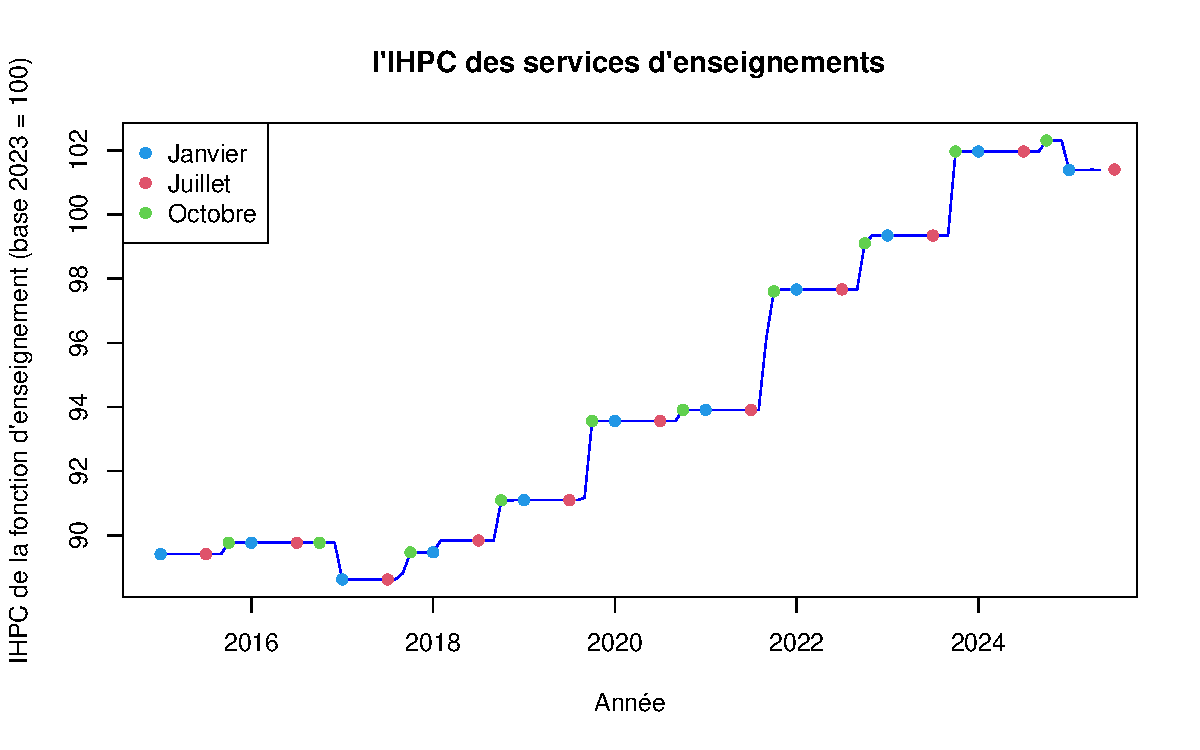
\includegraphics[width=0.95\textwidth]{graph de 2015 jav -2025 mai-1}
 	\caption{Visualisation de la série de janvier 2015 à mai 2025}
 	\label{fig:graph de 2015 jav -2025 mai-1}
 \end{figure}
 
 Lors de l'analyse de l'évolution de l'\IHPC{} nous remarquons que celui-ci a évolué d'environ \textbf{13,4\,\%} sur la période de \textit{janvier 2015 à mai 2025}. Une évolution marquée par la stagnation de l'indice sur certaines des périodes et une hausse brusque de ce dernier sur d'autres. Il faut aussi noter que la série n'est pas continue. En effet, sur certaines périodes, nous assistons à des chocs externes qui changent le cours normal de l'évolution de l'indice. La période \textit{décembre 2016} et \textit{janvier 2017} en est un parfait exemple. 
 
 Par ailleurs, la visualisation de la série révèle une \textit{tendance croissante} et une \textit{saisonnalité régulière} de l'IHPC des \textit{Services d'enseignement}. En effet, on remarque que l'indice croît à chaque rentré scolaire en octobre et se stabilise ensuite tout au long de l'année scolaire jusqu'en vacances (octobre-septembre). A chaque rentré,  les établissements révisent leurs tarifs dû généralement à l'inflation générale ---payement des salaires des enseignants, électricité, eau..., quand les prix augmentent dans l'économie, ils répercutent donc cette hausse sur les frais de scolarité---, et au faite que la demande en éducation est forte et inélastique --- même quand les frais augmentent, les familles continuent de payer--- . La révision des tarifs reste telle jusqu'à la fin de l'année scolaire en question, raison de la stabilité de l'indice après chaque rentrée. Le graphe ci-dessous illustre parfaitement nos dires.
  
 \textbf{Remarque:} La visualisation de la fonction \textbf{decompose à modèle additif} nous permet juste d'appuyer nos dires. 
 
 

\begin{figure}[H]
	\centering
	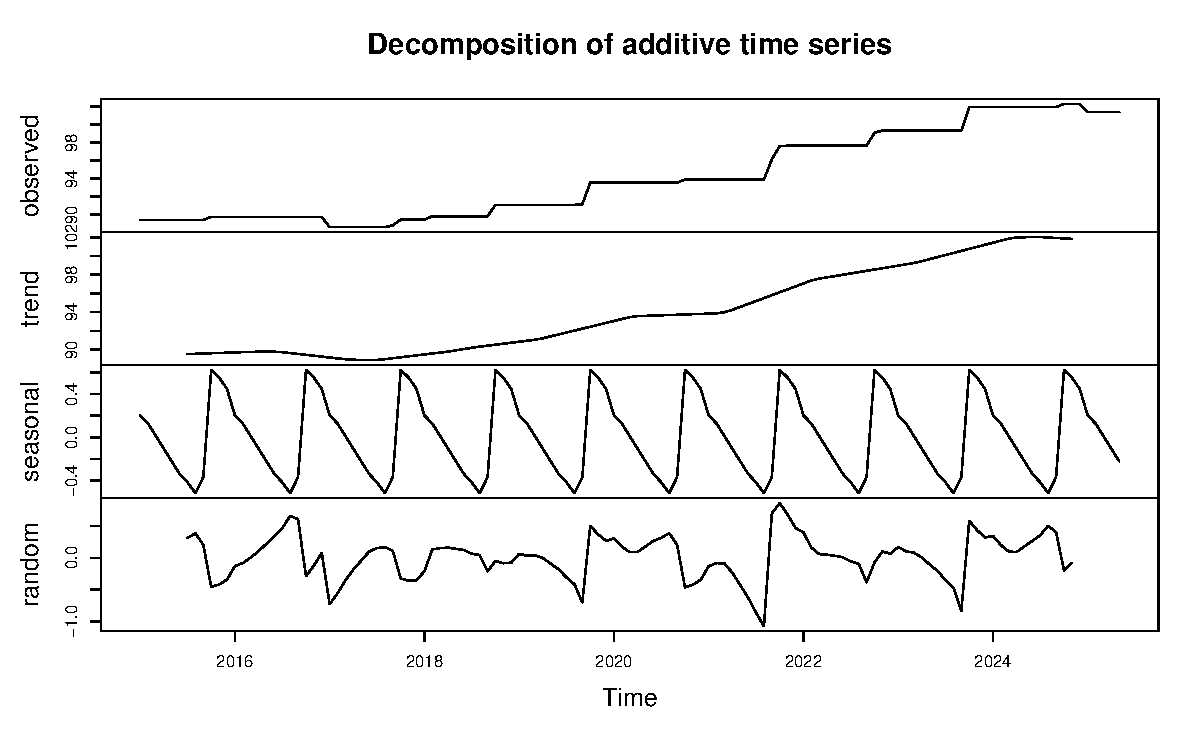
\includegraphics[width=0.95\textwidth]{graph_saisonnalité_tendance-1}
	\caption{Visualisation de la saisonnalité et de la tendance}
	\label{fig:graph_saisonnalité_tendance-1}
\end{figure}
L'observation du ci-dessus, met à évidence une saisonnalité régulière de la série et une tendance non linéaire.  


L’ensemble des moments de la série ne sont pas indépendants dans le temps. En effet, avec une tendance croissante, la moyenne de l'indice varie d'une année à une autre. Le code   \textbf{ breakpoints(base1 ~ 1)} renvoie  cinq breakpoints correspondants aux dates:  \textbf{mars 2018, septembre 2019, aout 2021, septembre 2023}. 


 Dans la suite de l'étude de la fonction, afin que nos prévisions soient plus proche de la réalité, nous nous pencherons sérieusement sur la nature de la saisonnalité( est-elle additive, multiplicative ou mixte ?) et celle de la tendance (est-elle linéaire?). 
 Il faut noter que les amplitudes de variations saisonnière ne restent pas constantes tout au long de la période 2015-2025, elles croient dans le temps. 
  
 \chapter{Prévision par lissage exponentiel}
 
 \section{ Discussion du lissage exponentiel approprié}
 
 
 \subsection{Discussion du lissage choisi}
 
Le modèle de Holt-Winters est une méthode de lissage exponentiel triple qui permet de prévoir des séries chronologiques en tenant compte du niveau, de la tendance et de la saisonnalité, ce qui le rend adapté à notre série. On opte pour la méthode saisonnière additive car les amplitudes de variations ne varient pas exponentiellement. 
Pour le lissage, nos choix des coefficients a été fait manuellement en se basant sur la nature de notre série. En effet: 

---pour le niveau $\alpha$, nous avons choisit une valeur très proche de 1: $\mathbf{0{,}99}$ car le modèle accorde une grande importance aux observations récentes due aux révisions des frais de scolarités à chaque rentrée. 

--- pour la tendance $\beta$, le choix a été fait sur une valeur proche de 0: $\mathbf{0{,}125}$ car cette dernière est lente et stable.  

--- pour la saisonnalité $\gamma$,  le choix a été $\mathbf{1}$ car les coefficients saisonniers sont entièrement mis à jour à chaque période. 

\begin{table}[H]
	\centering
	\centering
\centering
\begin{tabular}[t]{lrl}
\toprule
Paramètre & Valeur & Interprétation\\
\midrule
\cellcolor{gray!10}{alpha (Niveau)} & \cellcolor{gray!10}{0.990} & \cellcolor{gray!10}{Grande réactivité aux observations récentes}\\
beta (Tendance) & 0.125 & Tendance lente et stable\\
\cellcolor{gray!10}{delta (Saisonnalité)} & \cellcolor{gray!10}{1.000} & \cellcolor{gray!10}{Saisonnalité entièrement mise à jour}\\
\bottomrule
\end{tabular}


	\caption{Coefficients de lissage retenus pour Holt-Winters}
	\label{tab:coeff_lissage}
\end{table}


\subsection{Le modèle de Holt-Winters additif}

 
 Le modèle de Holt-Winters additif avec saisonnalités d'ordre $p$ 
 propose une prévision à l'horizon $h$, au vu de $Y_1, Y_2, \ldots, 
 Y_T$, sous la forme :
 
 \begin{equation}
 	\hat{Y}_T(h) = a_T + b_T h + S_{T-p+h}
 	\label{eq:hw_additif}
 \end{equation}
 
 Avec les formules de mise à jour suivantes :
 
 \begin{align}
 	a_T &= \alpha \left[Y_T - S_{T-p}\right] + 
 	(1 - \alpha)(a_{T-1} + b_{T-1}) 
 	\label{eq:hw_niveau} \\
 	b_T &= \beta \left[a_T - a_{T-1}\right] + 
 	(1 - \beta)\, b_{T-1} 
 	\label{eq:hw_tendance} \\
 	S_T &= \delta \left[Y_T - a_T\right] + 
 	(1 - \delta)\, S_{T-p} 
 	\label{eq:hw_saison}
 \end{align}
 
 où $\alpha$, $\beta$, $\delta$ sont des constantes choisies dans 
 $[0, 1]$.
 
 

 Pour initialiser $a_p$, $b_p$ et $\hat{S}_j$, $j = 1, \ldots, p$,
 on utilise les moindres carrés sur les points $(t, Y_t)$,
 $t = 1, \ldots, p + h$, $h \geq 1$ \citep{somda2026}.
 
 \begin{equation}
 	b_p = \frac{12}{p(p^2 - 1)}
 	\left[
 	\sum_{k=1}^{p} k Y_k - \frac{p(p+1)}{2}\,\bar{Y}_p
 	\right]
 	\label{eq:b_p}
 \end{equation}
 
 \begin{equation}
 	a_p = \bar{Y}_p + \frac{p-1}{2}\, b_p
 	\label{eq:a_p}
 \end{equation}
 
 \begin{equation}
 	S_j = Y_j - a_p - b_p\,\frac{j - p}{p}, \quad j = 1, \ldots, p
 	\label{eq:S_j}
 \end{equation}
 
 avec $\bar{Y}_p = \dfrac{1}{p} \displaystyle\sum_{k=1}^{p} Y_k$
 
  
 \section{ Prévision des indices de prix de juin à septembre 2025}
 
 \subsection{ Les paramètres initiaux}
 
 Par le biais des formules d'initialisation, nous avons calculé les paramètres initiaux à savoir celui du niveau, la pente et les coefficients saisonniers. Les résultats sont présentés dans les tableaux suivants: 
 
 
 \begin{table}[H]
 	\centering
 	\centering
\centering
\begin{tabular}[t]{lr}
\toprule
Paramètre & Valeur\\
\midrule
\cellcolor{gray!10}{Niveau initial} & \cellcolor{gray!10}{89.68500}\\
Pente initiale & 0.03357\\
\bottomrule
\end{tabular}


 	\caption{Paramètres initiaux (le niveau et la pente) (année 2015) --- Lissage HOLT-WINTERS}
 	\label{tab:params_initiaux}
 \end{table}
 
 \begin{table}[H]
 	\centering
 	\centering
\centering
\begin{tabular}[t]{lr}
\toprule
Mois & Coefficient\\
\midrule
\cellcolor{gray!10}{Jan} & \cellcolor{gray!10}{-0.242800}\\
Fév & -0.245600\\
\cellcolor{gray!10}{Mar} & \cellcolor{gray!10}{-0.248400}\\
Avr & -0.251200\\
\cellcolor{gray!10}{Mai} & \cellcolor{gray!10}{-0.254000}\\
Jun & -0.256700\\
\cellcolor{gray!10}{Jul} & \cellcolor{gray!10}{-0.259500}\\
Aoû & -0.262300\\
\cellcolor{gray!10}{Sep} & \cellcolor{gray!10}{-0.265100}\\
Oct & 0.087700\\
\cellcolor{gray!10}{Nov} & \cellcolor{gray!10}{0.084900}\\
Déc & 0.082100\\
\cellcolor{gray!10}{Somme} & \cellcolor{gray!10}{-2.030994}\\
\bottomrule
\end{tabular}


 	\caption{Coefficients saisonniers initiaux (année 2015) --- Lissage HOLT-WINTERS}
 	\label{tab:tab:coeff_saisonniers_init}
 \end{table}
 
 
 \subsection{La mise à jour (les coefficients finaux)}
 
 Là on applique les formules de la mise à jour afin d'avoir les coefficients finaux. 
 
 \begin{table}[H]
 	\centering
 	\centering
\centering
\begin{tabular}[t]{lr}
\toprule
Paramètre & Valeur\\
\midrule
\cellcolor{gray!10}{Niveau final} & \cellcolor{gray!10}{101.650800}\\
Pente finale & -0.008548\\
\bottomrule
\end{tabular}


 	\caption{Paramètres finaux --- Lissage HOLT-WINTERS}
 	\label{tab: params_finaux}
 \end{table}
 
 \begin{table}[H]
 	\centering
 	\centering
\centering
\begin{tabular}[t]{lr}
\toprule
Mois & Coefficient\\
\midrule
\cellcolor{gray!10}{Jan} & \cellcolor{gray!10}{-0.264800}\\
Fév & -0.266500\\
\cellcolor{gray!10}{Mar} & \cellcolor{gray!10}{-0.268500}\\
Avr & -0.246400\\
\cellcolor{gray!10}{Mai} & \cellcolor{gray!10}{0.152000}\\
Jun & 0.075400\\
\cellcolor{gray!10}{Jul} & \cellcolor{gray!10}{0.067800}\\
Aoû & -0.244800\\
\cellcolor{gray!10}{Sep} & \cellcolor{gray!10}{-0.254300}\\
Oct & -0.259800\\
\cellcolor{gray!10}{Nov} & \cellcolor{gray!10}{-0.261400}\\
Déc & -0.263100\\
\cellcolor{gray!10}{Somme} & \cellcolor{gray!10}{-2.034397}\\
\bottomrule
\end{tabular}


 	\caption{Coefficients saisonniers finaux --- Lissage HOLT-WINTERS}
 	\label{tab:coeff_saisonniers_finaux}
 \end{table}
 
 
 
 \subsection{Etude de la composante résiduelle}
 
 Pour l'analyse de cette dernière, cinq tests statistiques ont été menés sur la composante afin de vérifier si elle est un bruit blanc ou pas. 
 Les résultats de ces tests sont présentés en dessous : 
 
 \begin{table}[H]
 	\centering
 	\centering
\centering
\begin{tabular}[t]{lrrl}
\toprule
Test & Statistique & p-value & Décision\\
\midrule
\cellcolor{gray!10}{Centralité (Student)} & \cellcolor{gray!10}{-0.2752} & \cellcolor{gray!10}{0.7836021} & \cellcolor{gray!10}{Ne pas rejeter \$H\_0\$}\\
Homoscédasticité (Breusch-Pagan) & 1.2301 & 0.2673845 & Ne pas rejeter \$H\_0\$\\
\cellcolor{gray!10}{Indépendance résidus / t (cor.test)} & \cellcolor{gray!10}{-0.2579} & \cellcolor{gray!10}{0.7969292} & \cellcolor{gray!10}{Ne pas rejeter \$H\_0\$}\\
Autocorrélation (Ljung-Box) & 15.1178 & 0.2350559 & Ne pas rejeter \$H\_0\$\\
\cellcolor{gray!10}{Normalité (Shapiro-Wilk)} & \cellcolor{gray!10}{0.5537} & \cellcolor{gray!10}{0.0000000} & \cellcolor{gray!10}{Rejeter \$H\_0\$}\\
\bottomrule
\end{tabular}


 	\caption{Résultats des tests statistiques sur la composante résiduelle}
 	\label{tab:resultats_tests_holt_winters}
 \end{table}
 
 \textbf{ Interprétation des résultats}
 

 
 \begin{itemize}
 	\item \textbf{Test de student (centralité)} --- la \textbf{$p_value$}= 0.783, alors on ne rejette pas  à \textbf{ 95\,\%} de certitude l'hypothèse $H_0$  selon laquelle La moyenne des résidus est nulle(µ = 0). En d'autres termes, les résidus ne renvoient aucune information.
 	
 	\item \textbf{Test de Breusch-Pagan (Homoscédasticité)} --- la \textbf{$p_value$}= 0.27, alors on ne rejette pas à \textbf{ 95\,\%} de confiance l'hypothèse $H_0$ selon laquelle les résidus sont homoscédastiques. Autrement dit, leur variance est constante sur la période d'étude.
 	
 	\item \textbf{Indépendance résidus/ t (cor.test)} --- la \textbf{$p_value$}= 0.8, alors on ne rejette pas  au \textbf{ seuil de 5\,\%} l'hypothèse $H_0$ selon laquelle il n'existe pas une corrélation entre résidus et la variable explicative $t$.
 	Les résidus sont indépendants du temps.
 	
 	\item \textbf{Test de Ljung-Box (Autocorrélation)} ---la \textbf{$p_value$}= 0.235, alors on ne rejette pas au \textbf{ seuil de 5\,\%} l'hypothèse $H_0$ selon laquelle il n'existe pas d'autocorrélation des résidus.
 	En d'autres terme, les résidus ne sont pas corrélées entre elles.
 	
 	\item \textbf{Test de Shapiro-Wilk (Normalité)} --- la \textbf{$p_value$}= 0.0000, alors on rejette au \textbf{ seuil de 5\,\%} l'hypothèse $H_0$ selon laquelle les résidus suivent une loi normale. 
 \end{itemize}
 
 
 Au regard de ces résultats, on admet que les erreurs ne sont pas de bruit blanc. 
 Mais nous jugeons bon le modèle pour les prévisions.
 
 \subsection{Prévisions des indices de prix de juin à septembre 2025}
 
 Tableau comparatif des indices prédites et ceux observés.
 
 \begin{table}[H]
 	\centering
o 	\centering
\centering
\begin{tabular}[t]{lrrr}
\toprule
Mois & Valeur\_prévue & Valeur\_observée & Erreur\\
\midrule
\cellcolor{gray!10}{Juin 2025} & \cellcolor{gray!10}{101.7176} & \cellcolor{gray!10}{101.3877} & \cellcolor{gray!10}{-0.3299}\\
Juillet 2025 & 101.7015 & 101.4046 & -0.2969\\
\cellcolor{gray!10}{Août 2025} & \cellcolor{gray!10}{101.3804} & \cellcolor{gray!10}{101.4046} & \cellcolor{gray!10}{0.0242}\\
Septembre 2025 & 101.3623 & 101.4210 & 0.0587\\
\bottomrule
\end{tabular}


 	\caption{Prévisions et valeurs observées (Juin--Septembre 2025) --- Lissage HOLT-WINTERS}
 	\label{tab: prevision_vs_observe_HOLT_WINTERS}
 \end{table}
 
 
 Nous remarquons que les prévisions sont très proches des valeurs observées, même si des écarts subsistent. Les prévisions obtenues sont légèrement inférieures sur certains mois et supérieures sur d'autres aux valeurs réellement observées, ce qui
 signifie que le modèle s'adapte au fur et à mesure. Cependant, en se basant sur la nature de notre fonction, l'indice prédite devrait être constante de juin à septembre (toute chose étant égale par ailleurs). En effet, la période de prévision correspond aux vacances, une période pendant laquelle aucun justement n'est faite sur les frais de scolarité de l'année 2024-2025 car les classes sont fermées. Même si les écarts entres les valeurs prédites sont à $10^{-1}$ près, pour des prix à des millions de CFA, le modèle reste à désirer.  
 
 
  Le graphique de la prévision.
  
 \begin{figure}[H]
 	\centering
 	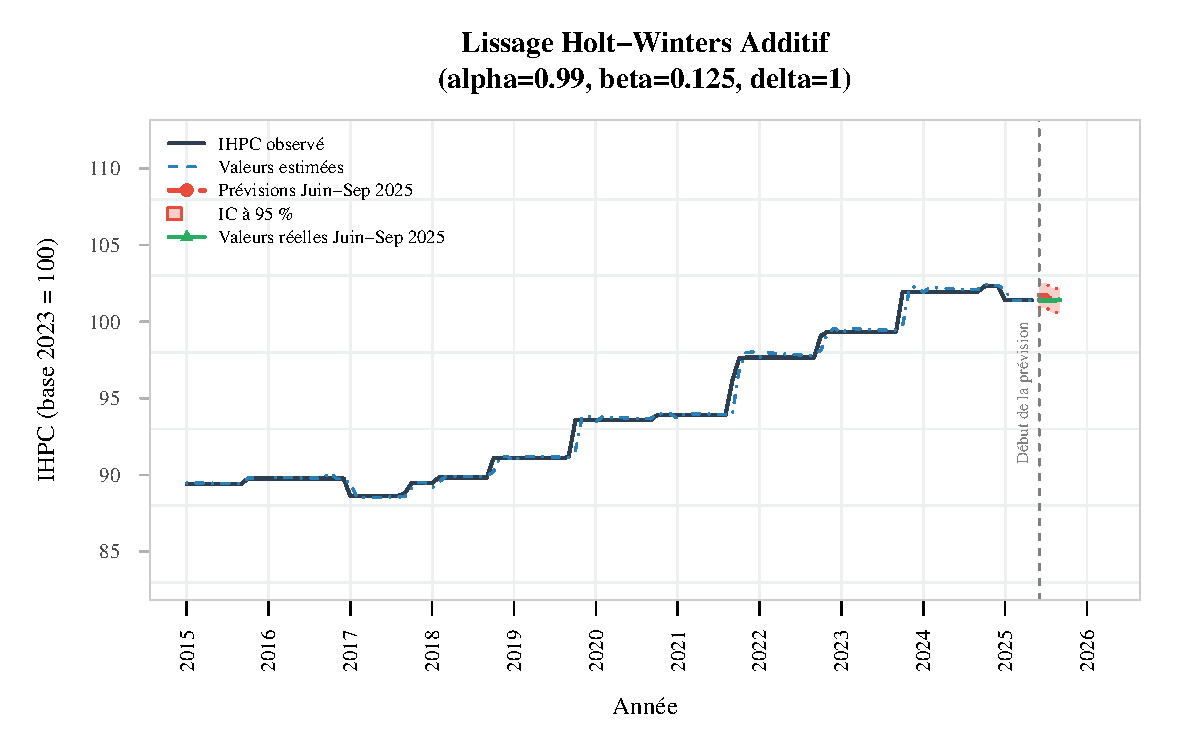
\includegraphics[width=0.95\textwidth]{graphe_prevision_lissage-1}
 	\caption{Visualisation de la prédiction}
 	\label{fig:graphe_prevision_lissage-1}
 \end{figure}
 
 Le graphique montre que la courbe d’ajustement suit de très près la série réelle, confirmant la bonne qualité du modèle.
 
 \section{L'erreur quadratique moyenne (EQM)}
 
 L’erreur quadratique moyenne (EQM) sert à mesurer la précision d’un modèle. En d'autres termes, si l’EQM est faible, cela signifie que les prédictions du modèle sont proches des valeurs réelles, dans le cas contraire cela indique que le modèle commet de grandes erreurs.
 
 Sa formule: 
 
 \begin{equation}
 	EQM = \frac{1}{n} \sum_{t=1}^{n} e_t^2
 \end{equation}
 
 avec $\quad e_t = (y_t - \hat{y}_t)$
 
 \begin{itemize}
 	\item $y_t$ : les observations réelles aux dates $t$
 	\item $\hat{y}_t$ : les observations prédites aux dates $t$
 \end{itemize}
 
 \begin{table}[H]
 	\centering
 	\centering
\centering
\begin{tabular}[t]{lr}
\toprule
Indicateur & Valeur\\
\midrule
\cellcolor{gray!10}{EQM} & \cellcolor{gray!10}{0.050248}\\
RMSE & 0.224160\\
\bottomrule
\end{tabular}


 	\caption{Erreur quadratique moyenne --- Lissage HOLT-WINTERS}
 	\label{tab:eqm_HOLT_WINTERS}
 \end{table}
 
 \textbf{L'EQM} calculée est égale à \textbf{0,050248}, une valeur très proche de \textbf{0} et sa racine carré \textbf{RMSE= 0.22} , ce qui indique que le modèle approche au mieux les valeurs réelles observées. En d'autres termes, cela signifie que les prévisions s’écartent en moyenne d’environ 0.22 points d’indice des valeurs observées.
 
 \section{La couverture moyenne}
 
 Servant à évaluer la fiabilité des intervalles de confiances, le tableau ci-dessous donne la couverture des données prédites sur la période juin-septembre 2025 de l'IHPC de la  fonction Enseignement. 
 
 
  \begin{table}[H]
 	\centering
 	\centering
\centering
\begin{tabular}[t]{lrrrl}
\toprule
Mois & Valeur prédite & Borne inf. IC & Borne sup. IC & Dans l'IC\\
\midrule
\cellcolor{gray!10}{Juin 2025} & \cellcolor{gray!10}{101.7176} & \cellcolor{gray!10}{100.9409} & \cellcolor{gray!10}{102.4943} & \cellcolor{gray!10}{Oui}\\
Juillet 2025 & 101.7015 & 100.9247 & 102.4782 & Oui\\
\cellcolor{gray!10}{Août 2025} & \cellcolor{gray!10}{101.3804} & \cellcolor{gray!10}{100.6037} & \cellcolor{gray!10}{102.1571} & \cellcolor{gray!10}{Oui}\\
Septembre 2025 & 101.3623 & 100.5856 & 102.1390 & Oui\\
\cellcolor{gray!10}{Couverture globale} & \cellcolor{gray!10}{NA} & \cellcolor{gray!10}{NA} & \cellcolor{gray!10}{NA} & \cellcolor{gray!10}{100\% (4/4)\}}\\
\bottomrule
\end{tabular}


 	\caption{Couverture de l'intervalle de confiance --- Lissage HOLT-WINTERS}
 	\label{tab:couverture_ic_HOLT_WINTERS}
 \end{table}
 
 Après calcul, on remarque toutes les prévisions sont dans l'intervalle de confiance à \textbf{95\,\%} de certitude , la couverture affiche donc  une proportion de \textbf{100\,\%}.
 
 
 \chapter{Prévision par décomposition simple}
 
 \section{ Discussion de l'approche }
 \subsection{ Discussion de la saisonnalité et de son modèle}
  L'évolution des prix des services éducatifs ne stagnent pas tout au long de la période d'étude. En effet, il passe de \textbf{88,62} (valeur minimale) à \textbf{102,31} (valeur maximale), soit une augmentation d'environ \textbf{10,8\,\%} de janvier 2015 à décembre 2022. Cette évolution de l'indice s'est faite de façon modérée avec des amplitudes de variations saisonnières qui ne diffèrent pas exponentiellement. Avec une telle évolution, le modèle additif serait le mieux adapté à notre série. Nous avons appliqué le test de \textbf{Buys-Ballot} dont le but est  vérifier si l'écart-type de la série est constant au cours des mois. Ce test intervient pour appuyer nos dires.
   
  \textbf{Méthode :} 
  
  - On regroupe les données par période (tous les mois de janvier, tous les mois de février…).
  
  - On calcule pour chaque période la moyenne et l’écart-type.
  
  \textbf{Interprétation:} 
  
  - Si les écarts-types sont relativement similaires entre périodes alors la série est homoscédastique donc le modèle additif est valide.
  
  - Si certains mois présentent un écart-type nettement plus élevé alors la série est hétéroscédastique donc on rejette le modèle additif.
  
  \begin{table}[H]
  	\centering
  	\centering
\centering
\begin{tabular}[t]{lrr}
\toprule
Mois & Moyenne & Ecart\_Type\\
\midrule
\cellcolor{gray!10}{Jan} & \cellcolor{gray!10}{91.69} & \cellcolor{gray!10}{3.11}\\
Feb & 91.73 & 3.08\\
\cellcolor{gray!10}{Mar} & \cellcolor{gray!10}{91.73} & \cellcolor{gray!10}{3.08}\\
Apr & 91.73 & 3.08\\
\cellcolor{gray!10}{May} & \cellcolor{gray!10}{91.73} & \cellcolor{gray!10}{3.08}\\
Jun & 91.73 & 3.08\\
\cellcolor{gray!10}{Jul} & \cellcolor{gray!10}{91.73} & \cellcolor{gray!10}{3.08}\\
Aug & 91.73 & 3.08\\
\cellcolor{gray!10}{Sep} & \cellcolor{gray!10}{92.05} & \cellcolor{gray!10}{3.36}\\
Oct & 93.03 & 3.71\\
\cellcolor{gray!10}{Nov} & \cellcolor{gray!10}{93.07} & \cellcolor{gray!10}{3.78}\\
Dec & 93.07 & 3.78\\
\bottomrule
\end{tabular}


  	\caption{Évolution de la moyenne et de sigma chaque mois-- Test de Buys-Ballot}
  	\label{tab:modele_additif}
  \end{table}
  
  L'analyse du tableau ci-dessus révèle en effet que les écart-types des observations sont pratiquement similaires entre les différents mois. Alors le modèle \textbf{additif} est accepté. 
  \textbf{Sa formule est la suivante:} 
  
  \[
  Y_t = T_t + S_t + \varepsilon_t
  \] 


 \textbf{Explication des termes:}
 
- $Y_t$ : la série observée à la période t

- $T_t$ : la composante de tendance

- $S_t$ : la composante saisonnière

- $\varepsilon_t$ :  les résidus 


 \subsection{ Discussion de la tendance et de son modèle}
   La visualisation du graphe de la fonction \textbf{decompose à modèle additif} vue plus haut, met en évidence une tendance croissante.
  Quatre modèles de régression ont été envisagés pour la modélisation de la tendance : la régression linéaire, quadratique, cubique et enfin par une fonction polynomiale de degré 4. Après plusieurs essais comparatifs, le modèle polynomial de degré 4 a été retenu avec un \textbf{ R² ajusté de 0.9624}. Autrement dit, cela signifie que près de \textbf{96,24\,\%} des variations de l'indice des prix des services d'enseignement sont expliquées par le modèle avec un niveau de confiance de \textbf{95\,\%}. 
  Ce pendant, concernant les coefficients, seule la constante est significative  au seuil \textbf{5\,\%}.
 
  Le choix de ce modèle repose sur le fait qu'il ajuste au mieux les valeurs observées contrairement aux autres modèles.
  
  Il faut noter que l’analyse des résidus a mis en évidence une hétéroscédasticité et une auto-corrélation. Malgré ces limites, le modèle est jugé suffisamment robuste pour poursuivre l’étude.
  
  \textbf{La formule du modèle cubique: }
  \[
  Y_t = \beta_0 + \beta_1 t + \beta_2 t^2 + \beta_3 t^3 + \beta_4 t^4 
  \]
  
 Explications : 
 
 - $Y_t$ : L'indice au temps t.
 
 - $\beta_0$  : constante.
 
 - $\beta_1t$ : effet linéaire du temps.
 
 - $\beta_2t^2$ : effet quadratique (courbure).
 
 - $\beta_3t^3$ : effet cubique (qui permet de modéliser des changements de pente plus complexes).
 
 - $\beta_4t^4$ :il capte les les changements très complexe de la tendance.
 
 
 
 
 
 \section{ Décomposition et Modélisation de la série}
 Commençons par le calcul de la moyenne mobile.
 
  \subsection{ Calcul de la moyenne mobile}
  Une moyenne mobile \textbf{MM} d’ordre \textbf {k} est une technique de lissage des séries temporelles qui consiste à calculer, pour chaque instant \textbf{t}, la moyenne pondérée des \textbf{k} observations successives entourant \textbf{t}. L’ordre \textbf{k} correspond donc au nombre de valeurs prises en compte dans la fenêtre de calcul. 
  
  \textbf{Sa formule de calcul est la suivante:}
  
  \[
  MM_t = \sum_{i=-m_1}^{m_2} \theta_i \, X_{t+i}
  \]
  
 - $MM_t$ : moyenne mobile au temps t.
 
 - $X_{t+i}$ : valeur de la série au temps t+i.
 
 - $\theta_i$ : poids attribué à chaque observation (satisfaisant $\sum \theta_i$=1).
 
 - $m_1+m_2+1=k$ : taille de la fenêtre, c’est-à-dire l’ordre de la moyenne mobile.
 
 
 Nous avons appliqué une moyenne mobile d’ordre \textbf{$k=12$}, 
 en attribuant un poids $\tfrac{1}{24}$ aux deux extrémités de la fenêtre 
 et un poids uniforme $\tfrac{1}{12}$ aux 10 valeurs centrales. 
 Ce choix permet de conserver la propriété de normalisation 
 $\left(\sum \theta_i = 1\right)$ 
 et limite l’influence des valeurs extrêmes. 
 Ainsi, la moyenne mobile obtenue reflète mieux la tendance centrale de la série.
 
\begin{figure}[H]
	\centering
	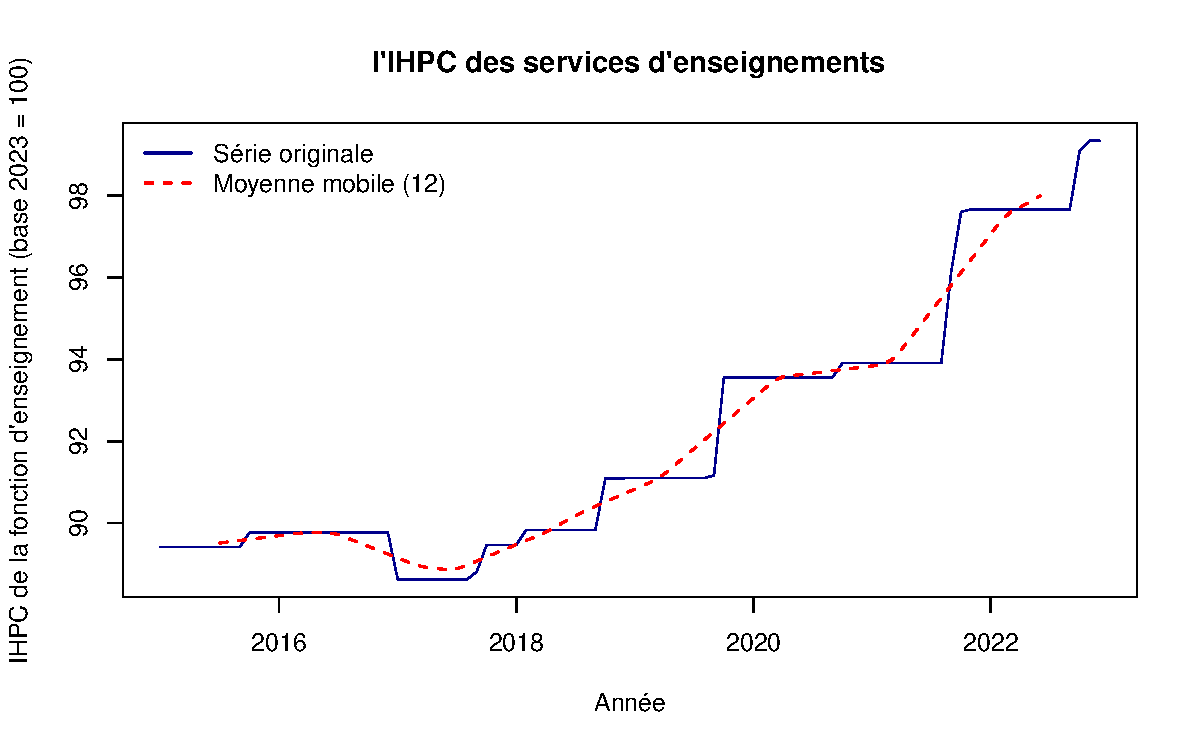
\includegraphics[width=0.95\textwidth]{graph_moyenne_mobiel-1}
	\caption{Visualisation de la moyenne mobile d'ordre 12}
	\label{fig:moyenne_mobiel}
\end{figure}
 
 \subsection{ Détermination des coefficients saisonniers}
 
 Après le calcul de la moyenne mobile, nous avons d'abord déterminer grossièrement les coefficients saisonniers en passant d'abord par la détermination de la différence saisonnière ($\Delta_t$) en soustrayant la moyenne mobile d’ordre p ($MM_t$) aux observations de la série($Y_t$): 
 
 \[
 \Delta_t = Y_t - MM_p(Y_t)
 \]
 
 Après le calcul de $\Delta_t$, nous passons à l'estimation brute des coefficients saisonniers proprement dite par médiane des  $\Delta_t$:
 
 \[
 S'_j = \text{médiane}\{\Delta_k \mid k \equiv j \ (\text{mod } p)\}, \quad j = 1, \ldots, p
 \]
 
 
 En fin, nous ajustons les  coefficients pour que leur somme soit nulle:
 
 \[
 \hat{S}_j = S'_j - \frac{1}{p} \sum_{k=1}^{p} S'_k
 \]
 
 Les résultats sont présentés dans le tableau ci-dessous: 
 
 
 \begin{table}[H]
 	\centering
 	\centering
\centering
\begin{tabular}[t]{llr}
\toprule
  & Mois & Coefficient\\
\midrule
\cellcolor{gray!10}{Jan} & \cellcolor{gray!10}{Jan} & \cellcolor{gray!10}{0.0610}\\
Feb & Feb & 0.1463\\
\cellcolor{gray!10}{Mar} & \cellcolor{gray!10}{Mar} & \cellcolor{gray!10}{0.0381}\\
Apr & Apr & -0.0704\\
\cellcolor{gray!10}{May} & \cellcolor{gray!10}{May} & \cellcolor{gray!10}{-0.2028}\\
Jun & Jun & -0.2526\\
\cellcolor{gray!10}{Jul} & \cellcolor{gray!10}{Jul} & \cellcolor{gray!10}{-0.2754}\\
Aug & Aug & -0.3610\\
\cellcolor{gray!10}{Sep} & \cellcolor{gray!10}{Sep} & \cellcolor{gray!10}{-0.1760}\\
Oct & Oct & 0.3204\\
\cellcolor{gray!10}{Nov} & \cellcolor{gray!10}{Nov} & \cellcolor{gray!10}{0.4157}\\
Dec & Dec & 0.3567\\
\cellcolor{gray!10}{} & \cellcolor{gray!10}{Somme} & \cellcolor{gray!10}{0.0000}\\
\bottomrule
\end{tabular}


 	\caption{Les coefficients saisonniers}
 	\label{tab:coeff_saisonniers_decomposition}
 \end{table}
 
 
 \subsection{ Détermination de la tendance}
 
 Une fois les coefficients saisonniers obtenus, on procède à une correction de la série en retranchant la saisonnalité. On obtient \textbf{la série CVS: Série Corrigée des Variations Saisonnières}:
 \[
 Y_{ij}^{CVS} = Y_{ij} - \hat{S}_j \quad ; \quad j = 1, \ldots, p \ ; \ i = 1, \ldots, n
 \]
 
 On procède ensuite à l’estimation de la tendance par une régression en une \textbf{fonction cubique}:
 \[
 Y_t = \beta_0 + \beta_1 t + \beta_2 t^2 + \beta_3 t^3 + \beta_4 t^4
 \]
 
 
 Le tableau ci-dessous donne les coefficients de la fonction ainsi que leur \textbf{$p_value$}:
 
 \begin{table}[H]
 	\centering
 	\centering
\centering
\begin{tabular}[t]{llrrl}
\toprule
  & Variable & Coefficient & p-value & Décision\\
\midrule
\cellcolor{gray!10}{1} & \cellcolor{gray!10}{(Intercept)} & \cellcolor{gray!10}{89.86724} & \cellcolor{gray!10}{0.000000} & \cellcolor{gray!10}{Significatif}\\
2 & t & -0.05061 & 0.278311 & Non significatif\\
\cellcolor{gray!10}{3} & \cellcolor{gray!10}{I(t\textasciicircum{}2)} & \cellcolor{gray!10}{0.00054} & \cellcolor{gray!10}{0.780720} & \cellcolor{gray!10}{Non significatif}\\
4 & I(t\textasciicircum{}3) & 0.00003 & 0.387995 & Non significatif\\
\cellcolor{gray!10}{5} & \cellcolor{gray!10}{I(t\textasciicircum{}4)} & \cellcolor{gray!10}{0.00000} & \cellcolor{gray!10}{0.286465} & \cellcolor{gray!10}{Non significatif}\\
value & Test de Fisher (global) & 609.01680 & 0.000000 & Modèle globalement significatif\\
\bottomrule
\end{tabular}


 	\caption{Significativité du modèle polynomial}
 	\label{tab:resultats_modele_polynomial}
 \end{table}
 
 Au niveau des coefficients seule la \textbf{$p_value$} de la constante est significative
  au \textbf{seuil de 5\,\%}. En outre, la \textbf{$p_value$} du test de \textbf{Fisher} est significative à  \textbf{ 95\,\%} de confiance. Autrement dit, le modèle ajuste au mieux les valeurs observées à \textbf{ 95\,\%} de confiance.
 
 
 
 \section{ Analyse de la composante résiduelle et interprétation des résultats}
 
 Pour l'analyse de la composante résiduelle, nous avons mené cinq tests statistiques sur celle-ci afin de vérifier si elle est un bruit blanc ou pas. 
 Les résultats de ces tests sont présentés en dessous : 
 
 
 \begin{table}[H]
 	\centering
 	\centering
\centering
\begin{tabular}[t]{lrrl}
\toprule
Test & Statistique & p-value & Décision\\
\midrule
\cellcolor{gray!10}{Centralité (Student)} & \cellcolor{gray!10}{0.0000} & \cellcolor{gray!10}{1.0000000} & \cellcolor{gray!10}{Ne pas rejeter \$H\_0\$}\\
Homoscédasticité (Breusch-Pagan) & 30.6092 & 0.0000037 & Rejeter \$H\_0\$\\
\cellcolor{gray!10}{Indépendance résidus / t (Pearson)} & \cellcolor{gray!10}{0.0000} & \cellcolor{gray!10}{1.0000000} & \cellcolor{gray!10}{Ne pas rejeter \$H\_0\$}\\
Autocorrélation (Ljung-Box) & 205.4095 & 0.0000000 & Rejeter \$H\_0\$\\
\cellcolor{gray!10}{Normalité (Shapiro-Wilk)} & \cellcolor{gray!10}{0.9873} & \cellcolor{gray!10}{0.4875865} & \cellcolor{gray!10}{Ne pas rejeter \$H\_0\$}\\
\bottomrule
\end{tabular}


 	\caption{Les coefficients de la régression polynomiale}
 	\label{tab:resultats_tests_polynomiale}
 \end{table}
 
 \textbf{ Interprétation des résultats}
 
 
 
 \begin{itemize}
 	\item \textbf{Test de student (centralité)} --- la \textbf{$p_value$}= 1, alors on ne rejette pas  à \textbf{ 95\,\%} de certitude l'hypothèse $H_0$  selon laquelle La moyenne des résidus est nulle(µ = 0). En d'autres termes, les résidus ne renvoient aucune information.
 	
 	\item \textbf{Test de Breusch-Pagan (Homoscédasticité)} --- la \textbf{$p_value$}= 0.000, alors on rejette à \textbf{ 95\,\%} de confiance l'hypothèse $H_0$ selon laquelle les résidus sont homoscédastiques. Autrement dit, leur variance n'est pas constante sur la période d'étude.
 	 Cela indique que le modèle ne capture pas bien la dynamique de la variance 
 	
 	\item \textbf{Indépendance résidus/ t (cor.test)} --- la \textbf{$p_value$}= 1, alors on ne rejette pas  au \textbf{ seuil de 5\,\%} l'hypothèse $H_0$ selon laquelle il n'existe pas une corrélation entre résidus et les variables explicatives qui sont $t$, $t^2$, $t^3$, $t^4$.
 	En d'autres terme, les résidus sont indépendants des variables explicatives.
 	
 	
 	\item \textbf{Test de Ljung-Box (Autocorrélation)} ---la \textbf{$p_value$}= 0.000, alors on rejette au \textbf{ seuil de 5\,\%} l'hypothèse $H_0$ selon laquelle il n'existe pas d'autocorrélation des résidus.
 	En d'autres terme, les résidus sont corrélées entre elles. Ll reste une dépendance temporelle non expliquée par le modèle.
 	
 	\item \textbf{Test de Shapiro-Wilk (Normalité)} --- la \textbf{$p_value$}= 0.49, alors on ne rejette pas au \textbf{ seuil de 5\,\%} l'hypothèse $H_0$ selon laquelle les résidus suivent une loi normale. 
 \end{itemize}
 
 Ces résultats sont confirmés par les graphes suivants: 
 
 \begin{figure}[H]
 	\centering
 	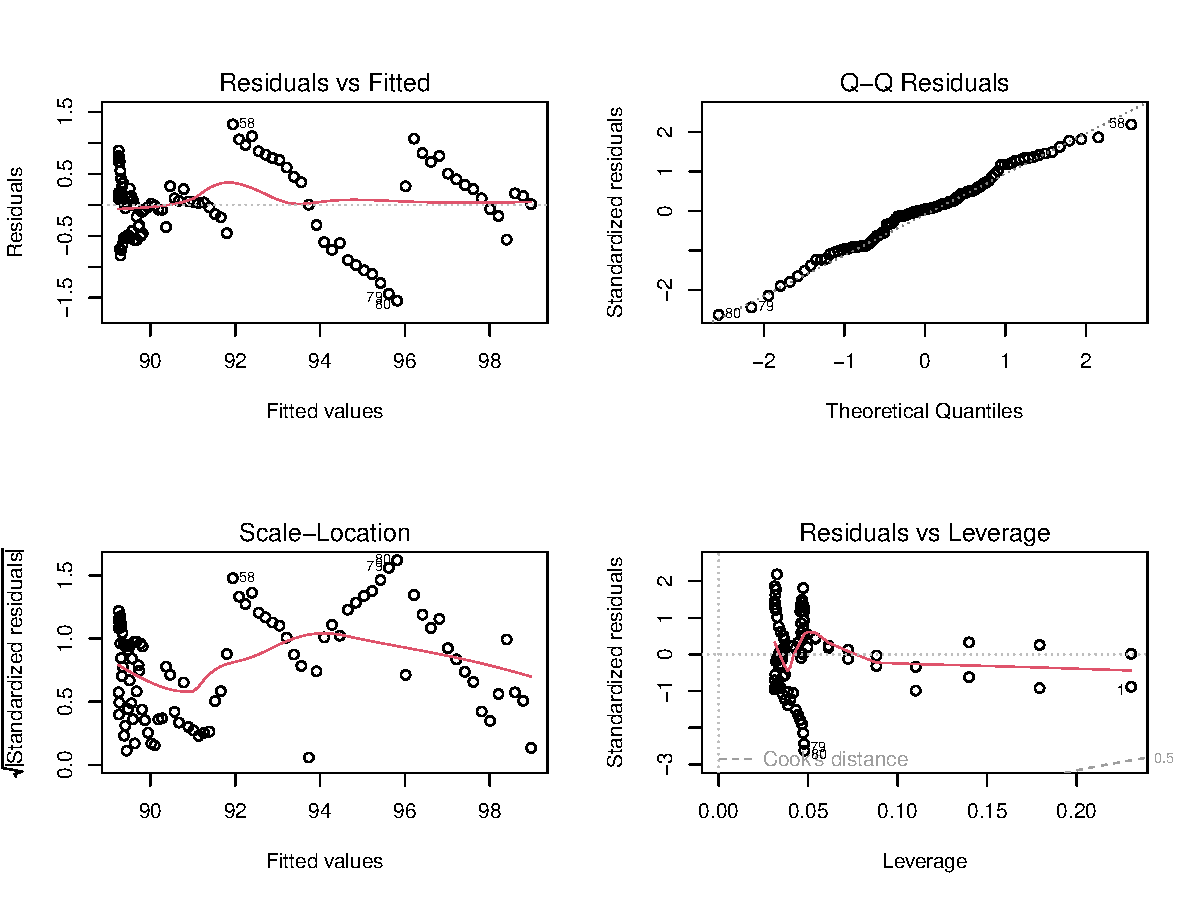
\includegraphics[width=0.95\textwidth]{graphe_diagnostic_lm_decomp}
 	\caption{ Visualisation du diagnostic du modèle polynomial}
 	\label{fig:diagnostic_lm_decomp}
 \end{figure}
  Le graphe \textbf{Residuals vs Fitted} renvoie que les erreurs oscillent autour de \textbf{0}, la ligne étant presque horizontale sur \textbf{$y=0$}.
  
  L'analyse du \textbf{Q-Q Residuals} met évidence le fait que les résidus sont normalement distribués. En effet, le bruit cache la \textbf{première bissectrice}.
  
  L'observation du \textbf{Scale-Location} confirme nos dires sur l'homoscédasticité car la ligne rouge est loin d'être horizontale: leur variance varie dans le temps.
  
 
 
 \begin{figure}[H]
 	\centering
 	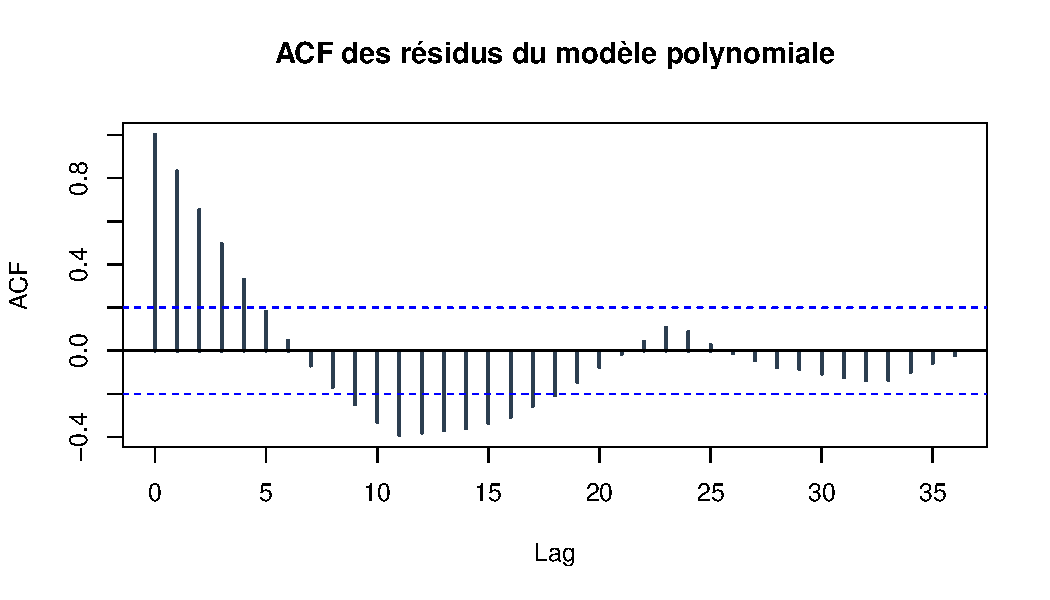
\includegraphics[width=0.95\textwidth]{graphe_acf_residus_decomp}
 	\caption{ Visualisation de l'ACF des résidus}
 	\label{fig:acf_residus_decomp }
 \end{figure}
 
 L'ACF met évidence une corrélation des erreurs.
 
 
 Les résidus étant auto-corrélées et leur variance n'étant pas constante dans le temps alors elles ne sont pas \textbf{bruit blanc}. 

 \section{ Interprétation des valeurs obtenues}
 Au regard des différents résultats obtenus nous jugeons le modèle acceptable pour une prévision malgré le fait que le bruit n'est pas blanc. 
 
 
 \section{ Prévision des indices des prix de juin à septembre 2025.}
 
 Le modèle devant servir de prédiction étant connu maintenant, passons à la prévision des indices de prix des services d'enseignement de janvier2023-septembre 2025.
 
 Tableau comparatif des indices prédites et ceux observés.
 
 \begin{table}[H]
 	\centering
 	\centering
\centering
\begin{tabular}[t]{rrr}
\toprule
Valeur\_prévue & Valeur\_observée & Erreur\\
\midrule
\cellcolor{gray!10}{102.3268} & \cellcolor{gray!10}{101.3877} & \cellcolor{gray!10}{-0.9391}\\
102.3073 & 101.4046 & -0.9027\\
\cellcolor{gray!10}{102.2141} & \cellcolor{gray!10}{101.4046} & \cellcolor{gray!10}{-0.8095}\\
102.3802 & 101.4210 & -0.9592\\
\bottomrule
\end{tabular}


 	\caption{Prévisions et valeurs obervées (Janvier2023-Septembre 2025) --- Décomposition}
 	\label{tab:prevision_vs_observe_décomposition}
 \end{table}
 
 Le graphique de la prévision: 
 
 \begin{figure}[H]
 	\centering
 	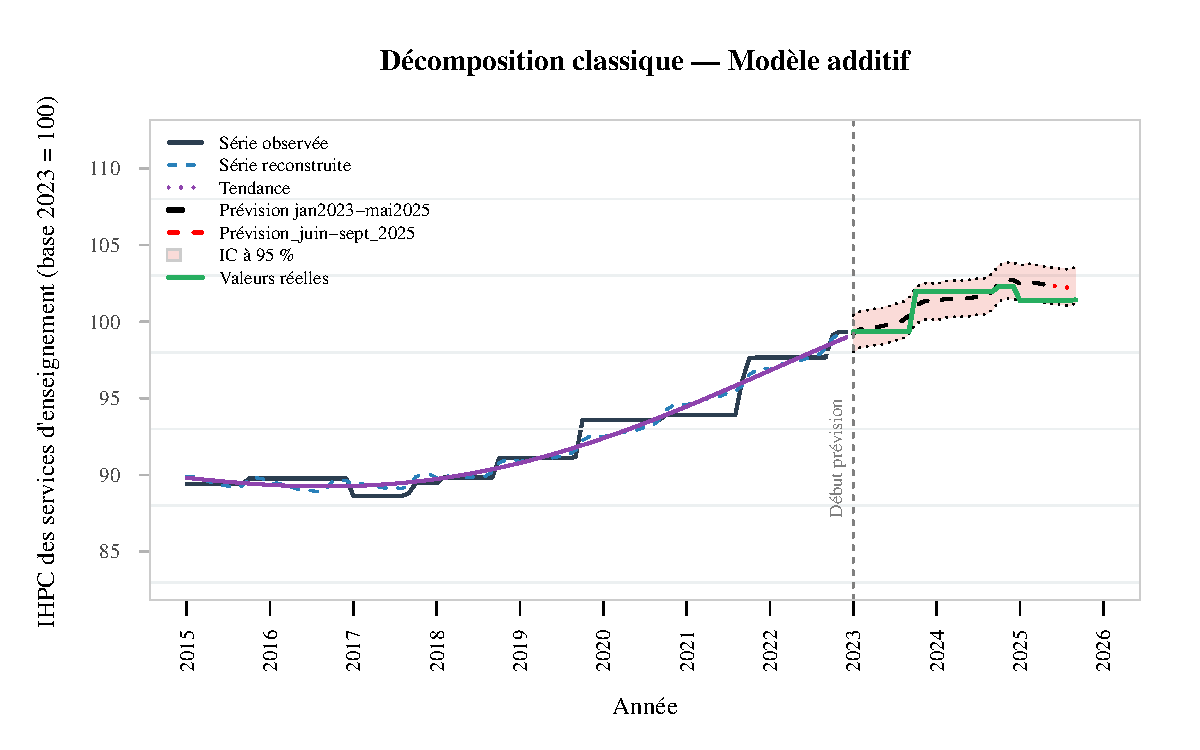
\includegraphics[width=0.95\textwidth]{graphe_prevision_decomp}
 	\caption{Visualisation de la prédiction}
 	\label{fig:prevision_decomp}
 \end{figure}
 
 Les prévisions par décomposition suivent la tendance polynomiale de degré 4 avec un intervalle de confiance à \textbf{95\,\%} de certitude qui s'adapte à chaque valeur prédite au cours du temps.
 On constate que la série réelle et prédite oscille tout en restant dans cet intervalle de
 confiance. Cependant, le modèle surestime l'indice et n'est pas stable sur période de juin à septembre 2025. Une approche qui laisse à désirer.
  
 
 
 
 \subsection{L'erreur quadratique moyenne (EQM)}
 

 
 \begin{table}[H]
 	\centering
 	\centering
\centering
\begin{tabular}[t]{lr}
\toprule
Indicateur & Valeur\\
\midrule
\cellcolor{gray!10}{EQM} & \cellcolor{gray!10}{0.818017}\\
RMSE & 0.904443\\
\bottomrule
\end{tabular}


 	\caption{Erreur quadratique moyenne --- Décomposition}
 	\label{tab:eqm_décomposition}
 \end{table}
 
 \textbf{L'EQM} calculée est égale à \textbf{0,81} de racine carré \textbf{0.9}, une valeur qui révèle que les valeurs réelles ont été bien ajustées. 
 
 \subsection{La couverture}
 

 \begin{table}[H]
 	\centering
 	\centering
\centering
\begin{tabular}[t]{rrrl}
\toprule
Valeur prédite & Borne inf. IC & Borne sup. IC & Dans l'IC\\
\midrule
\cellcolor{gray!10}{102.3268} & \cellcolor{gray!10}{101.1744} & \cellcolor{gray!10}{103.4792} & \cellcolor{gray!10}{Oui}\\
102.3073 & 101.1549 & 103.4597 & Oui\\
\cellcolor{gray!10}{102.2141} & \cellcolor{gray!10}{101.0617} & \cellcolor{gray!10}{103.3665} & \cellcolor{gray!10}{Oui}\\
102.3802 & 101.2278 & 103.5326 & Oui\\
\cellcolor{gray!10}{NA} & \cellcolor{gray!10}{NA} & \cellcolor{gray!10}{NA} & \cellcolor{gray!10}{100\% (4/4)\}}\\
\bottomrule
\end{tabular}


 	\caption{Couverture de l'intervalle de confiance --- Decomposition}
 	\label{tab:couverture_ic_decomposition}
 \end{table}
 
 Après calcul, on remarque toutes les prévisions sont dans l'intervalle de confiance donc la couverture affiche une proportion de \textbf{100\,\%} au seuil de \textbf{5\,\%}.
 
 
 \chapter{Modélisation par décomposition stochastique}
 
 \section{ Discussion de l'approche}
 
 Comme vue précédemment, notre série est une série saisonnière. Afin d'ajuster au mieux la série, nous vérifions de prime abord la stationnarité de cette dernière. Si elle ne l'est pas alors nous la différentions (différentions  tendancielle et/ou  saisonnière ) jusqu'à ce qu'elle soit stationnaire. Après quoi, nous déterminerons les coefficients du modèle \textbf{SARIMA (p,d,q)(P,D,Q)[s]} afin de faire des prévisions à long terme.
 
 
 
 
 \section{Méthodologie Box-Jenkins saisonnière : le modèle SARIMA}
 
 La modélisation \textbf{SARIMA} (\textbf{S}easonal \textbf{A}uto\textbf{R}egressive 
 \textbf{I}ntegrated \textbf{M}oving \textbf{A}verage) est une extension naturelle du 
 modèle ARIMA introduit par \textbf{BOX, George E.P. and JENKINS, Gwilym M.} pour les séries présentant une structure 
 saisonnière. Contrairement à l'ARIMA classique qui ne capture que la dépendance 
 temporelle à court terme, le SARIMA intègre une composante saisonnière permettant 
 de modéliser les régularités qui se répètent à intervalles fixes --- ici, à chaque 
 rentrée scolaire d'octobre. Il est noté \textbf{SARIMA$(p,d,q)(P,D,Q)[s]$}, où $s$ 
 désigne la période saisonnière (ici $s = 12$ pour des données mensuelles).
 
 L'équation générale du modèle s'écrit :
 
 \begin{equation}
 	\Phi_P(B^s)\,\phi_p(B)\,(1 - B^s)^D\,(1 - B)^d\,y_t
 	= \Theta_Q(B^s)\,\theta_q(B)\,\varepsilon_t
 	\label{eq:sarima}
 \end{equation}
 
 où les composantes se définissent comme suit :
 
 $y_t$ : La valeur de l'indice des prix observée à l'instant $t$.
 
 $B$ (Opérateur de retard / Backshift) : Par définition $By_t = y_{t-1}$ et 
 $B^s y_t = y_{t-s}$ (la valeur observée $s$ périodes auparavant).
 
 $(1 - B)^d$ : L'opérateur de différenciation tendancielle d'ordre $d$. Il 
 stationnarise la série en supprimant la tendance.
 
 $(1 - B^s)^D$ : L'opérateur de différenciation saisonnière d'ordre $D$. Il 
 supprime la composante saisonnière déterministe. Dans notre cas, $D = 0$ 
 car une seule différenciation tendancielle a suffi à rendre la série stationnaire.
 
 $\phi_p(B) = 1 - \displaystyle\sum_{i=1}^{p} \phi_i B^i$ : Le polynôme 
 autorégressif (AR) non saisonnier d'ordre $p$. Il modélise la dépendance de 
 $y_t$ vis-à-vis de ses $p$ valeurs passées.
 
 $\theta_q(B) = 1 - \displaystyle\sum_{j=1}^{q} \theta_j B^j$ : Le polynôme 
 de moyenne mobile (MA) non saisonnier d'ordre $q$. Il modélise l'influence 
 des $q$ erreurs d'estimation passées sur la valeur actuelle.
 
 $\Phi_P(B^s) = 1 - \displaystyle\sum_{i=1}^{P} \Phi_i B^{is}$ : Le polynôme 
 autorégressif saisonnier d'ordre $P$. Il capture la dépendance de $y_t$ 
 vis-à-vis de ses valeurs aux mêmes périodes des années précédentes.
 
 $\Theta_Q(B^s) = 1 - \displaystyle\sum_{j=1}^{Q} \Theta_j B^{js}$ : Le polynôme 
 de moyenne mobile saisonnier d'ordre $Q$. Il pondère l'influence des erreurs 
 saisonnières passées.
 
 $\varepsilon_t$ : Le Bruit Blanc, représentant les chocs aléatoires et 
 imprévisibles du marché à l'instant $t$.
 
 Cette approche permet de capturer simultanément la dynamique 
 à court terme et la structure saisonnière de la série, sans qu'il soit 
 nécessaire de modéliser explicitement la tendance puisque celle-ci est 
 supprimée par différenciation.
 
 
 
 
 
 
 
 
  \section{ Déssaisonalisation et stationnarisation de la série }
  
 
 La déssaisonalisation consiste à retrancher les coefficients saisonniers aux observations réelles afin d'avoir une série sans saisonnalité. Quant à la stationnarisation, elle permet de stabiliser la série afin de rendre l'ensemble de ses moments indépendants dans le temps. 
 
 Nous allons d'abord faire un premier test de Dickey-Fuller sur la série afin de voir son état.
 
 \subsubsection{Explication du test de Dickey-Fuller}
 
 A ce niveau nous avons procédé par le test de \textbf{Dickey-Fuller} intégré dans une fonction de base \textbf{du logiciel R} qui est : \textbf{adf.test(x, alternative = c("stationary", "explosive"))}. 
Le test de Dickey-Fuller  est utilisé pour vérifier si la série temporelle possède une racine unitaire. La présence de cette dernière signifie que la série n’est pas stationnaire et qu’elle suit une marche aléatoire.

 On part du modèle autorégressif simple (d'ordre 1):
 \[
  Y_t = \phi Y_{t-1} + \varepsilon_t
 \]
 
où :\begin{itemize}
 \item $Y_t$ est la série observée à la date $t$.

  \item $Y_{t-1}$ est la série observée à la date $t-1$.
 
 \item $\phi$ est le coefficient auto-régressif, il mesure l'influence de la valeur passée ($Y_{t-1}$) sur la valeur présente ($Y_t$).
 
\item $\varepsilon_t$ est un bruit .

\end{itemize}


Les deux tests statistiques se font sur $\phi$. L'interprétation pour les différentes valeurs de $\phi$ sont : 
\begin{itemize}
\item $\phi$ <1 : la série est stationnaire. Les chocs aléatoires s’atténuent avec le temps et la série reste autour d’une certaine moyenne.

\item  $\phi$ =1 : la série possède une racine unitaire. Chaque choc a un effet permanent, la série suit une marche aléatoire.

\item  $\phi$ >1 : la série est explosive. Les valeurs augmentent ou diminuent de plus en plus vite avec temps ($t$), la variance diverge.

 \item  $\phi$ <-1 :  la série est aussi explosive, mais avec des oscillations qui s’amplifient (elle change de signe à chaque pas).
\end{itemize}

En réécrivant cette équation sous forme de différences, on obtient ainsi: 
\[
\Delta Y_t =(\phi -1 ) Y_{t-1} + \varepsilon_t = \delta Y_{t-1} + \varepsilon_t
\]
 
 avec $\delta = \phi -1$
 
 Pour le test proprement dit, on a: 
 \begin{itemize}
 \item \textbf {Test avec alternative = "stationary"}
 On veut vérifier si la série est stationnaire ($\delta <0$).
 Les hypothèses du test sont: 
 \[
 H_0 : \delta = 0 \quad (\phi = 1,\ \mathrm{racine\ unitaire})
 \]
 
 \[
 H_1 : \delta < 0 \quad (|\phi| < 1,\ \mathrm{stationnaire})
 \] 
 
 \item \textbf {Test avec alternative = "explosive"}
 On veut vérifier si la série croît ou décroît exponentiellement avec le temps. En d'autres termes, on veut vérifier si la variance devient très grande à long terme($\delta >0$).
 Les hypothèses du test sont: 
 \[
 H_0 : \delta = 0 \quad (\phi = 1,\ \mathrm{racine\ unitaire})
 \]
 
 \[
 H_1 : \delta > 0 \quad (\phi > 1,\ \mathrm{explosif})
 \]
 

 \end{itemize}
 
 
 \subsubsection{Application du test}
 
 Nous avons appliqué un premier test de \textbf{Dickey-Fuller} avec les deux \textbf{alternatives: "explosive" et "stationary"}, la \textbf{$p_value$} dans les deux cas est supérieure à \textbf{0,05} signe de la présence d'une \textbf{racine unitaire: donc la série n'est pas stationnaire}. On a donc affaire à une série à tendance \textbf{stochastique}.
 
  \begin{table}[H]
 	\centering
 	\centering
\centering
\begin{tabular}[t]{llrrrl}
\toprule
Hypothèse\_nulle & Hypothèse\_alternative & Statistique & p-value & Lag & Décision\\
\midrule
\cellcolor{gray!10}{Série non stationnaire (phi = 1)} & \cellcolor{gray!10}{Explosive (phi > 1)} & \cellcolor{gray!10}{-1.4993} & \cellcolor{gray!10}{0.2166} & \cellcolor{gray!10}{4} & \cellcolor{gray!10}{Ne pas rejeter H\_0}\\
Série non stationnaire (phi = 1) & Stationnaire (phi < 1) & -1.4993 & 0.7834 & 4 & Ne pas rejeter H\_0\\
\bottomrule
\end{tabular}


 	\caption{Tests de Dickey-Fuller sur la série de janvier2015-décembre2022}
 	\label{tab:tests_stationnaire1_cvs}
 \end{table}
 
 
 
 On procède ensuite à une première \textbf{différenciation tendancielle d'ordre 1(d=1)}, elle consiste à soustraire la valeur précédente de la  série à sa valeur actuelle. \textbf{$d1_serie_cvs <- diff(base2, differences=1)
 $}: 
 avec 
 
 \begin{itemize}
 	\item $base2$ : la série de janvier 2015-Décembre 2022.
 	
 	\item $diff(base2, differences=1)$ : ici on effectue la différenciation tendancielle d'ordre d=1.
 	
 \end{itemize}
 Autrement dit, on transforme la série $Y_t$  en une nouvelle série $\Delta Y_t$  définie par : $\Delta Y_t=Y_t-Y_{t-1}$. L'objectif de cette différenciation est de stabiliser la moyenne et la variance dans le temps afin de rendre la série stationnaire. Après cette différenciation, on refait les mêmes tests pour vérifier la présence de la \textbf{racine unitaire}. Les résultats sont présentés dans le tableau ci-dessous: 
 	
 \begin{table}[H]
 	\centering
 	\centering
\centering
\begin{tabular}[t]{llrrrl}
\toprule
Hypothèse\_nulle & Hypothèse\_alternative & Statistique & p-value & Lag & Décision\\
\midrule
\cellcolor{gray!10}{Série non stationnaire (phi = 1)} & \cellcolor{gray!10}{Explosive (phi > 1)} & \cellcolor{gray!10}{-4.8357} & \cellcolor{gray!10}{0.99} & \cellcolor{gray!10}{4} & \cellcolor{gray!10}{Ne pas rejeter H\_0}\\
Série non stationnaire (phi = 1) & Stationnaire (phi < 1) & -4.8357 & 0.01 & 4 & Rejeter H\_0\\
\bottomrule
\end{tabular}


 	\caption{Tests de Dickey-Fuller augmenté sur la série différenciée}
 	\label{tab:tests_stationnaire2_cvs }
 \end{table}
 
 Nous avons 
 Le test avec \textbf{l'alternative : "stationary"} présente une \textbf{$p_value$}  \textbf{0,01 < 0,05} ce qui révèle que  $|\phi| < 1$ car l'hypothèse alternative selon laquelle $\delta < 0$ est acceptée. La \textbf{différenciation tendancielle d'ordre 1(d=1)} seule a suffit de rendre stationnaire la série, raison pour laquelle nous n'allons pas procéder à la \textbf{différenciation saisonnière d'ordre D} donc \textbf{D=0}.
 
 
 \section{Proposition du modèle SARIMA}
 
 La détermination du modèle part de la visualisation de  \textbf{l'ACF et du PACF} de la série  \textbf{différenciée}. Soient les graphes \textbf{ACF et du PACF} de la dite série: 
 
 \begin{figure}[H]
 	\centering
 	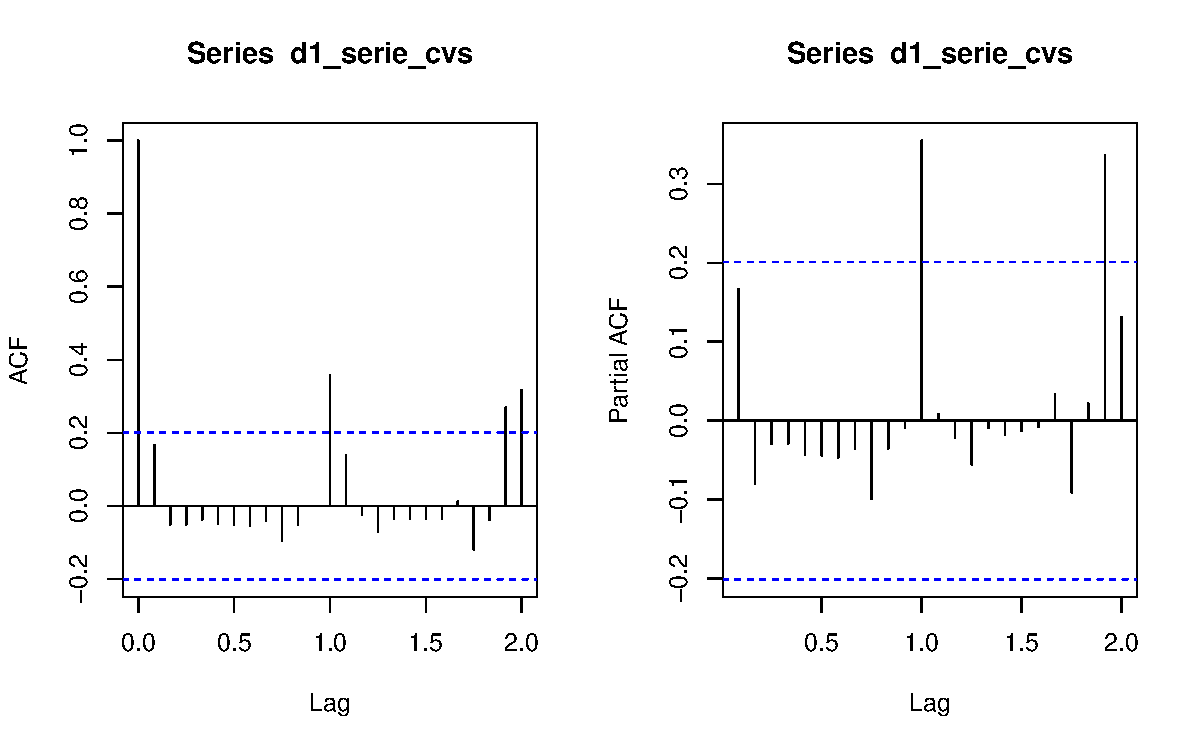
\includegraphics[width=0.95\textwidth]{graph ACF_PACF-1}
 	\caption{Visualisation de l'ACF et du PACF de la série différenciée}
 	\label{fig:graph ACF_PACF-1}
 \end{figure}
 
 La visualisation de ces deux graphes nous mène à considérer trois modèles SARIMA en considérant la saisonnalité. La formule générale est: 
 $arima(serie, order = c(p,d,q), seasonal = list(order = c(P,D,Q), period = 12))$
 
 Explication du choix des coefficients: 
 
 \begin{itemize}
 	
 	\item La partie non saisonnière $c(p,d,q)$ : 
 	
 	$p$ (auto-régression (AR)) Nombre de retards de la série utilisés
 	
 	$d$ Nombre de différenciation tendancielle de la série ici, $d=1$
 	
 	$q$ moyenne mobile (MA) Nombre d’erreurs passées utilisées
 	
 	\item La partie saisonnière $c(P,D,Q)$ :
 	
 	$P$ AR saisonnier
 	
 	$D$ Différenciation saisonnière ici, $D=0$
 	
 	$Q$ MA saisonnier
 	
 	\item $period = 12$ car les observations sont mensuelles
 	
 \end{itemize}
 
 
 On a: 
 
 \begin{itemize}
 	
 	\item  \textbf{$m1 <- arima(base2, order = c(2,1,2), seasonal = list(order = c(2,0,1), period = 12))$}
 	
 	
 	\item \textbf{$m2 <- arima(base2, order = c(0,1,0), seasonal = list(order = c(2,0,1), period = 12))$}
 	
 	
 	\item \textbf{$m3 <- arima(base2, order = c(2,1,0), seasonal = list(order = c(2,0,1), period = 12))$}.
 	
 \end{itemize}
 
 
 Pour choisir le meilleur modèle, nous les avons comparés par le biais des fonctions \textbf{AIC et BIC}, les résultats sont présentés dans le tableau ci-dessous: 
 
  \begin{table}[H]
  	\centering
  	\centering
\centering
\begin{tabular}[t]{lrr}
\toprule
Modèle & AIC & BIC\\
\midrule
\cellcolor{gray!10}{SARIMA(2,1,2)(2,0,1)[12]} & \cellcolor{gray!10}{99.0123} & \cellcolor{gray!10}{119.4434}\\
SARIMA(0,1,0)(2,0,1)[12] & 94.2674 & 104.4829\\
\cellcolor{gray!10}{SARIMA(1,1,1)(2,0,1)[12]} & \cellcolor{gray!10}{97.3930} & \cellcolor{gray!10}{112.7162}\\
\bottomrule
\end{tabular}


  	\caption{Comparaison des modèles ARIMA candidats (AIC / BIC)}
  	\label{tab:selection_arima }
  \end{table}
  
  Ces résultats révèlent que le meilleur modèle est \textbf{$arima(base2, order = c(0,1,0), seasonal = list(order = c(2,0,1), period = 12))$}. 
  
   \section{Étude des erreurs}
   
   Le modèle \textbf{ARIMA} étant connu, passons à l'analyse de la composante résiduelle. 
   
   \begin{figure}[H]
   	\centering
   	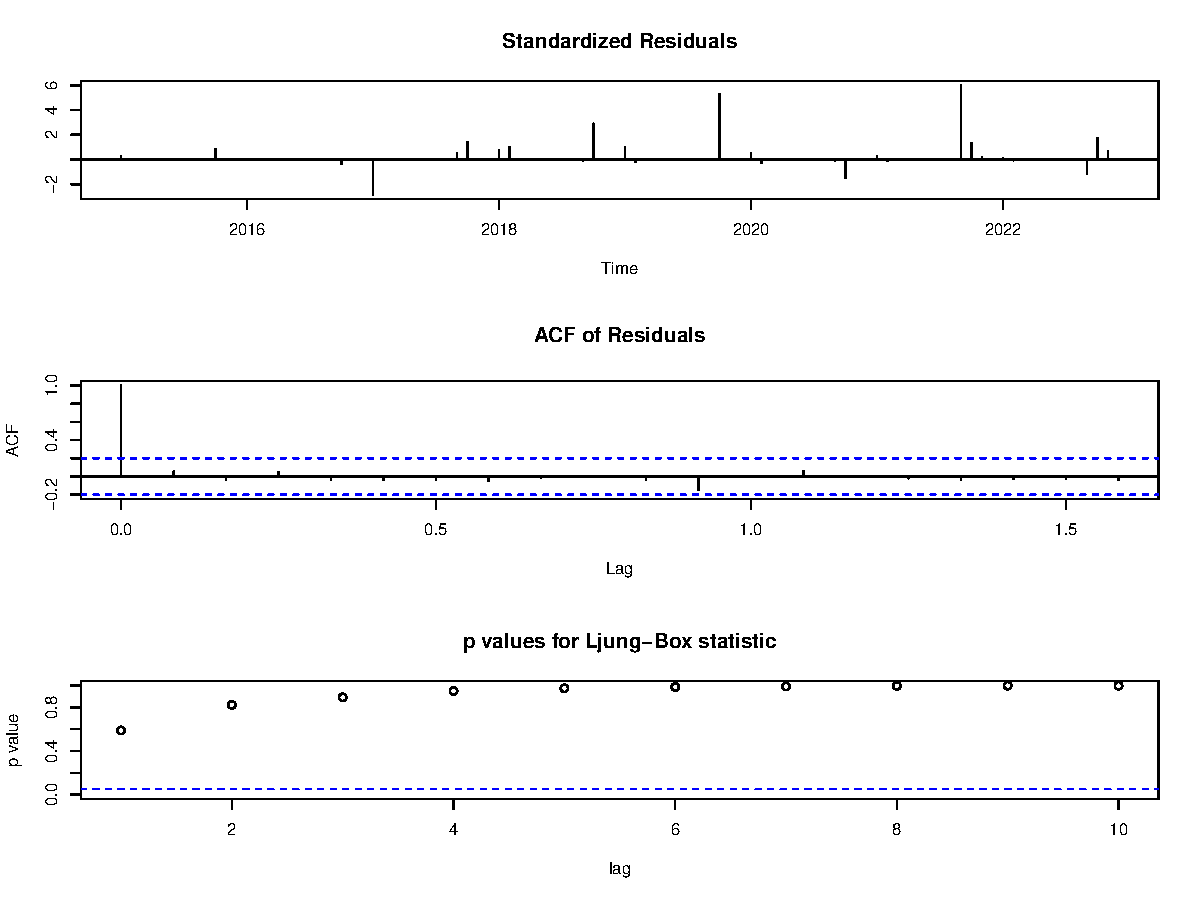
\includegraphics[width=0.95\textwidth]{graphe_diagnostic_sarima2}
   	\caption{Visualisation du diagnostic SARIMA(0,1,0)(2,0,1)[12]}
   	\label{fig:graphe_diagnostic_sarima2}
   \end{figure}
   
   L'image ci-dessus nous permet de visualiser trois graphes dont les interprétations sont: 
   \begin{itemize}
   	\item Le premier graphe \textbf{Standaedized Residuals} nous laisse voir que les erreurs oscillent autour de \textbf{0} avec une dispersion stable et peu de valeurs extrêmes ce qui suggère qu'elles n'apportent aucune information donc un modèle cohérent .
   	
   	\item La visualisation du deuxième graphique \textbf{ACF of Residuals} nous révèle qu'aucun pic n'est significatif signe que les erreurs ne sont pas auto-corrélées entre elles. 
   	
   	\item Le graphe \textbf{$p_value$ for Ljung-Box statistic} nous donne la $p_value$ du test statistique de \textbf{Ljung-Box}. 
   	---Le test de Ljung–Box est un outil statistique utilisé pour vérifier si les résidus d’un modèle de séries temporelles sont bien du bruit blanc, c’est-à-dire qu’ils ne présentent pas d’auto-corrélation significative. En d’autres termes, il sert à tester l’adéquation du modèle : si les résidus sont indépendants, le modèle explique correctement la structure de la série.---
   	Hypothèses du test:
   	Hypothèse nulle $H_0$ : Les résidus sont indépendants (pas d’auto-corrélation).
   	
   	Hypothèse alternative $H_1$ : Il existe au moins une auto-corrélation significative parmi les résidus (le modèle n’explique pas toute la dépendance).
   	
   	On visualise une $p_value >0.5$ qui est supérieure à \textbf{0.05} donc $H_0$ est acceptée ce qui suggère que le modèle explique correctement la série.
   	
   	\end{itemize}
 
 	En fin de compte, le \textbf{bruit est blanc.}
 	
 	\section{Interprétation des résultats}
 	Le \textbf{bruit étant blanc} pour le modèle le \textbf{SARIMA(0,1,0)(2,0,1)[12]} alors on l'accepte comme le meilleur modèle le \textbf{SARIMA} pouvant modéliser la série.
 	
 	\section{Prévision des indices de prix de janvier 2023 à septembre 2025 par le modèle SARIMA(0,1,0)(2,0,1)[12]}
 	
 	Le tableau ci-dessous est le tableau comparatif des indices prédites et ceux observés: 
 	
 	 \begin{table}[H]
 		\centering
 		\centering
\centering
\begin{tabular}[t]{rrr}
\toprule
Valeur\_prévue & Valeur\_observée & Erreur\\
\midrule
\cellcolor{gray!10}{102.1631} & \cellcolor{gray!10}{101.3877} & \cellcolor{gray!10}{-0.7754}\\
102.1403 & 101.4046 & -0.7357\\
\cellcolor{gray!10}{102.0547} & \cellcolor{gray!10}{101.4046} & \cellcolor{gray!10}{-0.6501}\\
102.6553 & 101.4210 & -1.2343\\
\bottomrule
\end{tabular}


 		\caption{Prévisions et valeurs observées --- Prévision SARIMA(0,1,0)(2,0,1)[12]
 			(Janvier 2023--Septembre 2025)}
 		\label{tab:prevision_vs_observe_arima}
 	\end{table}
 
 	Graphique de la prévision:
 	
 	
 	 \begin{figure}[H]
 		\centering
 		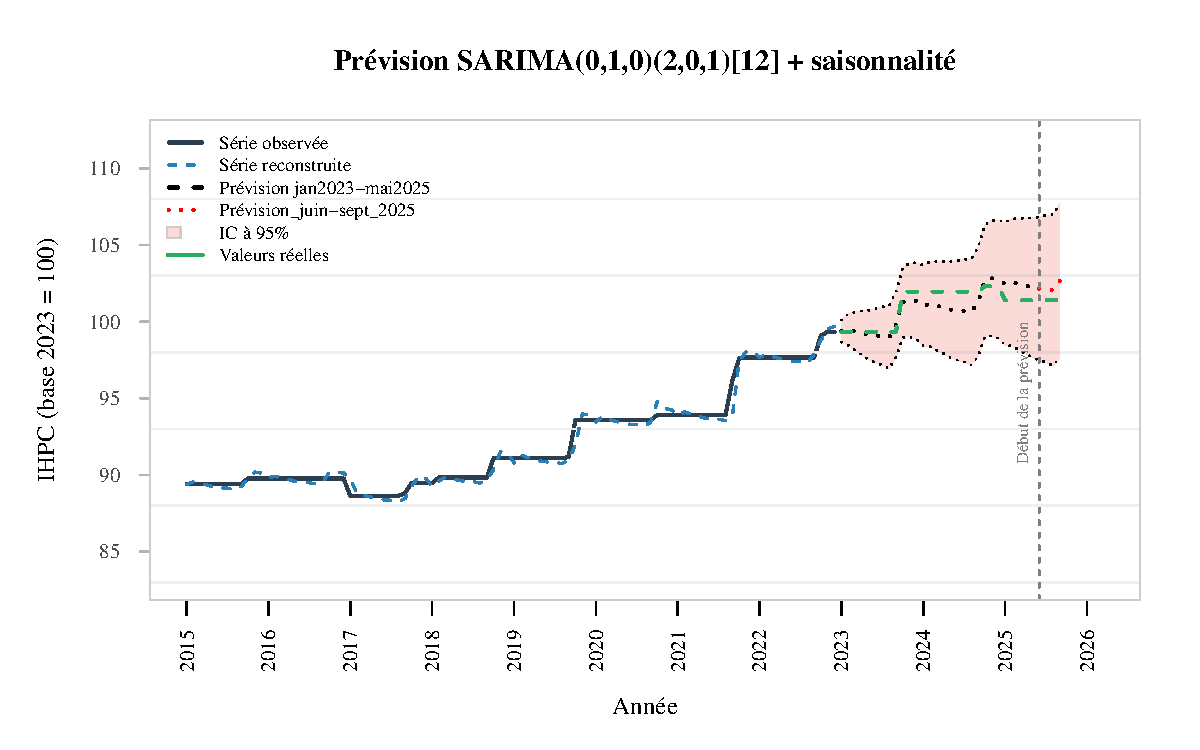
\includegraphics[width=0.95\textwidth]{graphe_prevision_arima}
 		\caption{Visualisation de la prévision}
 		\label{fig:graphe_prevision_arima}
 	\end{figure}
 	
 	On observe que l’intervalle de confiance à \textbf{95\,\%} s’élargit au cours du temps, ce qui montre que plus le temps
 	avance, plus le modèle devient moins performant dans ses prévisions. Ce dernier surestime également les valeurs réelles sur la période juin-septembre 2025. On constate que l'indice prédit au mois de septembre connait un saut, ce qui indique le modèle a bien capture la saisonnalité. En effet, La plupart des établissements publient leur tarifs dès le mois de septembre ce qui entraine un saut du l'ihpc de l'enseignement dès l fin du mois de septembre jusqu'en octobre( toute chose étant égale par ailleurs).
 	
 	\section{ Erreur Quadratique Moyenne}
 	
 	
 	\begin{table}[H]
 		\centering
 		\centering
\centering
\begin{tabular}[t]{lr}
\toprule
Indicateur & Valeur\\
\midrule
\cellcolor{gray!10}{EQM} & \cellcolor{gray!10}{0.772160}\\
RMSE & 0.878727\\
\bottomrule
\end{tabular}


 		\caption{Erreur quadratique moyenne--- SARIMA(0,1,0)(2,0,1)[12]}
 		\label{tab:eqm_sarima}
 	\end{table}
 	
  L'\textbf{EQM} calculée est égale à \textbf{0,772} de racine carré \textbf{0.878}, une valeur petite. Ce qui indique que le modèle \textbf{SARIMA(0,1,0)(2,0,1)[12]} approche bien les valeurs réelles observées.
  
  \section{ Couverture Moyenne}
  
  	\begin{table}[H]
  	\centering
  	\centering
\centering
\begin{tabular}[t]{rrrl}
\toprule
Valeur prédite & Borne inf. IC & Borne sup. IC & Dans l'IC\\
\midrule
\cellcolor{gray!10}{102.1631} & \cellcolor{gray!10}{101.3457} & \cellcolor{gray!10}{102.9805} & \cellcolor{gray!10}{Oui}\\
102.1403 & 101.3229 & 102.9577 & Oui\\
\cellcolor{gray!10}{102.0547} & \cellcolor{gray!10}{101.2373} & \cellcolor{gray!10}{102.8721} & \cellcolor{gray!10}{Oui}\\
102.6553 & 101.8380 & 103.4727 & Oui\\
\cellcolor{gray!10}{NA} & \cellcolor{gray!10}{NA} & \cellcolor{gray!10}{NA} & \cellcolor{gray!10}{100\% (4/4)\}}\\
\bottomrule
\end{tabular}


  	\caption{Couverture de l'intervalle de confiance à 95\,\% --- Prévision SARIMA(0,1,0)(2,0,1)[12]}
  	\label{tab:couverture_ic_sarima}
  \end{table}
  
  Après calcul, on remarque que toutes les prévisions sont dans l'intervalle de confiance donc la couverture affiche une proportion de \textbf{100\,\%} àn\textbf{95\,\%} de certitude.
  
  
  
  \chapter{Comparaison de la performance des modèles}
  
  \section{Comparaison des performances }
  
  La qualité des performances de prévision des trois approches sera jugée sur la base des \textbf{EQM}. Le tableau ci-dessous résume l'\textbf{EQM} de ces approches: 
  
  \begin{table}[H]
  	\centering
  	\centering
\centering
\begin{tabular}[t]{lrrl}
\toprule
Approche & EQM & RMSE & Couverture IC (95\textbackslash{}\%)\\
\midrule
\cellcolor{gray!10}{Lissage exponentiel (Holt-Winters)} & \cellcolor{gray!10}{0.050248} & \cellcolor{gray!10}{0.224160} & \cellcolor{gray!10}{100\%}\\
Décomposition classique & 0.818017 & 0.904443 & 100\%\\
\cellcolor{gray!10}{Modélisation stochastique (SARIMA)} & \cellcolor{gray!10}{0.772160} & \cellcolor{gray!10}{0.878727} & \cellcolor{gray!10}{100\%}\\
\bottomrule
\end{tabular}


  	\caption{Comparaison des approches}
  	\label{tab:comparaison_approche}
  \end{table}
  
  Ce tableau compare les performances des trois approches sur la période de prévision de juin à septembre 2025. Le modèle de lissage de \textbf{ lissage exponentiel par la méthode Holt-Winters} obtient l’\textbf{EQM} la plus faible (\textbf{0.05}), suivi du modèle \textbf{stochastique (SARIMA(0,1,0)(2,0,1)[12])} avec une \textbf{EQM = 0.772} , et enfin la décomposition classique qui
  présente l'\textbf{EQM} la plus élevée (\textbf{0.878}). Les trois modèles atteignent une couverture
  de \textbf{100\,\%} sur leurs intervalles de confiance à \textbf{95\,\%} de certitude.
  La meilleure approche est donc le \textbf{ lissage exponentiel par la méthode Holt-Winters} , en choisissant la plus petite  \textbf{EQM}  car il présente la plus faible \textbf{EQM} (0.05) et une couverture parfaite à \textbf{100\,\%}. Ce pendant, nous avons mené une série de prévisions sur les trois modèles et il ressort que le  modèle \textbf{stochastique (SARIMA(0,1,0)(2,0,1)[12])} est le modèle qui tient compte des caractéristiques de la série, à savoir sa saisonnalité et sa tendance à hausse ainsi que le saut de l'indice à chaque rentrée scolaire. Alors nous jugeons bon que le modèle  modèle \textbf{stochastique (SARIMA(0,1,0)(2,0,1)[12])} est la meilleur approche parmi les trois. 
  
  
  \section{Prévision sur le reste de l'année 2025}
  
  
  \begin{table}[H]
  	\centering
  	\centering
\centering
\begin{tabular}[t]{lr}
\toprule
Mois & Prévision\\
\midrule
\cellcolor{gray!10}{Octobre 2025} & \cellcolor{gray!10}{103.9351}\\
Novembre 2025 & 104.1020\\
\cellcolor{gray!10}{Décembre 2025} & \cellcolor{gray!10}{104.0432}\\
\bottomrule
\end{tabular}


  	\caption{La prévision d'Octobre-Décembre 2025}
  	\label{tab:prevision_arima_finale}
  \end{table}
  
  \begin{figure}[H]
  	\centering
  	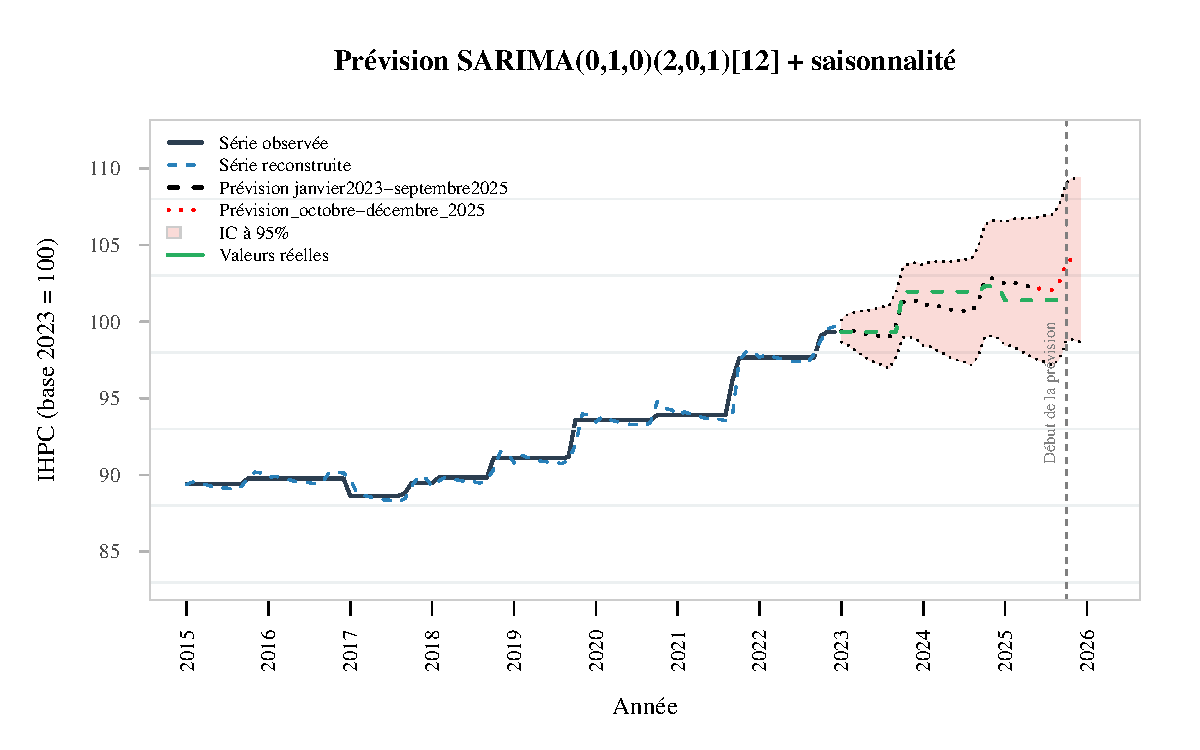
\includegraphics[width=0.95\textwidth]{graphe_prevision_arima_finale}
  	\caption{Visualisation  de la prévision d'octobre-décembre 2025 (SARIMA(0,1,0)(2,0,1)[12])}
  	\label{fig:graphe_prevision_arima_finale}
  \end{figure}
  
   Les prévisions d'octobre à décembre 2025 indiquent une poursuite à la hausse de l’indice des prix des services d'enseignement. Toute chose étant égale par ailleurs, les prévisions du modèle reflètent l'évolution naturelle de la fonction à savoir un saut des prix des services d'enseignement à chaque rentrée scolaire.
% ============================================================
%  CONCLUSION>      
% ============================================================

\chapter*{Conclusion}
\addcontentsline{toc}{chapter}{Conclusion}
\markboth{Conclusion}{Conclusion}


Ce travail avait pour objectif d’analyser et de modéliser l’évolution de l’\IHPC{} des services d’enseignement au Burkina Faso de janvier 2015 à mai 2025, afin d’en produire des prévisions jusque en décembre 2025.
Dans un premier temps, l’analyse de la série a révélé une tendance globalement croissante, ajustée par un polynôme de degré 4 présentant un $R^2$ de 0,98. Une saisonnalité marquée a également été observée, se manifestant principalement à chaque rentrée scolaire d’octobre par des sauts brusques de l’indice et une stagnation de celui ci au court de l'année scolaire.

Trois méthodes de modélisation ont ensuite été comparées sur la période de juin à septembre 2025. Il ressort de cette comparaison que le  modèle \textbf{stochastique (SARIMA(0,1,0)(2,0,1)[12])} s’est révélé le plus performant, avec une \EQM = 0,772 . Ce choix tient au fait qu'en plus de tenir compte de la saisonnalité, le modèle ajuste à bien la tendance croissante de l'indice avec des écarts qui laisse à désirer la qualité du modèle.



"\textbf{Il n'y a pas de statistiques fiables, seulement des statisticiens fiables}" \textbf{George Bernard SHAW}


% Synthèse des principaux résultats
% Meilleur modèle retenu et justification
% Limites de l'étude
% Perspectives

\newpage


% ============================================================
%  BIBLIOGRAPHIE
% ============================================================

\cleardoublepage
\addcontentsline{toc}{chapter}{Bibliographie}
\nocite{*}
\bibliographystyle{apalike}
\bibliography{references}


% ============================================================
%  ANNEXES
% ============================================================

\cleardoublepage
\addcontentsline{toc}{chapter}{Annexes}
\appendix



\end{document}